\chapter{圆锥曲线}
远在古希腊时代,人们就开始研究一个平面和一个正瞬
锥的截线的性质,并且获得了丰硕的成果,这些截线分别有
椭圆、抛物线和双曲线,并统称为圆锥曲线,在第二章
附录里,我们已用球面切线长相等原理证明了它们分别具有
如下几何特征.

椭圆有两个焦点$F_1,F_2$, 对椭圆上任一点$P$有
\[\overline{PF_1}+\overline{PF_2}=\text{常数}\]

双曲线有两个焦点$F_1,F_2$, 对双曲线上任一点$P$有
\[\overline{PF_1}-\overline{PF_2}=\text{常数}\]

抛物线有一个焦点,对抛物线上任一点$P$到焦点$F$与到
一定直线$\ell$的距离$d$相等,即
\[\overline{PF}:d=1\]

这一章,我们将要根据上述圆锥曲线的几何特性来定义
椭圆、双曲线和抛物线,建立它们在平面直角坐标系中的标
准方程,并利用标准方程进一步研究圆锥曲线其它的几何特
性.

\section{圆锥曲线的标准方程及其性质}
\subsection{椭圆的标准方程和形状}
\begin{blk}
    {定义} 平面内与两定点的距离之和等于常数(这常数必
须大于两定点间的距离)的点的轨迹叫做椭圆.这两定点叫
做椭圆的\textbf{焦点}.两焦点间的距离叫做\textbf{焦距}.
\end{blk}

下面,我们根据椭圆的定义来建立椭圆的方程.

设$F_1$、$F_2$是椭圆的两个焦点,取射线$F_1F_2$作为$X$轴
的正半轴,$\overline{F_1F_2}$的垂直平分线作为$Y$轴(图6.1).设
焦距$\overline{F_1F_2}=2c\; (c>0)$,则
\[F_1(-c,0),\qquad F_2(c,0)\]

\begin{figure}[htp]
    \centering
    \begin{tikzpicture}[>=latex]
\draw[->](-2.5,0)--(2.5,0)node[right]{$X$};
\draw[->](0,-2)--(0,2)node[right]{$Y$};
\draw[thick](0,0) ellipse [x radius=2, y radius=1.25];        
\tkzDefPoints{-1.56/0/F_1, 1.56/0/F_2, 1/1.08/P}
\tkzDrawSegments[thick](F_1,P P,F_2)
\tkzLabelPoints[below](F_1,F_2)
\tkzLabelPoints[above](P)
\node at (0,0)[below left]{$O$};
    \end{tikzpicture}
    \caption{}
\end{figure}


设$P(x,y)$是椭圆上的任一点,
它到$F_1$、$F_2$的距离之和等于常数
$2a\; (a>0)$, 则
\[\overline{PF_1}+\overline{PF_2}=2a\]
由求两点的距离公式得
\[\sqrt{(x+c)^2+y^2}+\sqrt{(x-c)^2+y^2}=2a\]
去根号,整理得
\begin{equation}
    (a^2-c^2)x^2+a^2y^2=a^2(a^2-c^2)
\end{equation}
因$\overline{PF_1}+\overline{PF_2}>\overline{F_1F_2}$, 所以$a>c,\; a^2-c^2>0$, 
设$a^2-c^2=b^2\; (b>0)$, 代入(6.1)式得
\[b^2x^2+a^2y^2=a^2b^2\]
两边同除$a^2b^2$得
\begin{equation}
 \boxed{\frac{x^2}{a^2}+\frac{y^2}{b^2}=1}   
\end{equation}
这就是说,椭圆上任一点的坐标都满足方程(6.2); 反过来,
设$P(x_1,y_1)$的坐标满足方程(6.2), 则
\[\frac{x_1^2}{a^2}+\frac{y_1^2}{b^2}=1\]
\[y^2_1=b^2\left(1-\frac{x^2_1}{a^2}\right)=(a^2-c^2)\left(1-\frac{x^2_1}{a^2}\right)\]
于是
\[\begin{split}
    \overline{PF_1}&=\sqrt{(x_1+c)^2+y^2_1}\\
    &=\sqrt{(x_1+c)^2+(a^2-c^2)\left(1-\frac{x^2_1}{a^2}\right)}\\
    &=\sqrt{a^2+2cx_1+\frac{c^2}{a^2}x^2_1}\\
    &=\left|a+\frac{c}{a}x_1\right|
\end{split}\]
由$\frac{x_1^2}{a^2}+\frac{y_1^2}{b^2}=1$,可推知
$\frac{x_1^2}{a^2}\le 1$,$|x_1|\le a$.

又因$c<a$,所以$\frac{c}{a}<1$,$\left|\frac{c}{a}x_1\right|<a$
,$a+\frac{c}{a}x_1>0$,因此:
\begin{equation}
    \overline{PF_1}=a+\frac{c}{a}x_1
\end{equation}
同理可证,
\[\overline{PF_2}=a-\frac{c}{a}x_1\]
所以:$\overline{PF_1}+\overline{PF_2}=2a$

这就是说,坐标满足方程(6.2)的点$P$也一定在椭圆上,由以
上证明,所以方程(6.2)是所求的椭圆方程,并把方程(6.2)
叫做\textbf{椭圆的标准方程}.

下面,用椭圆的标准方程来研究椭圆的几何形状.

首先,由于方程(6.2)中只含有$x,y$的平方,故把一
个坐标变号,对于方程没有影响,这就表明:如果$M(x,y)$
在椭圆上,那么,$M_1(x,-y)$, $M_2(-x,-y)$, $M_3(-x,
y)$各点也都在椭圆上,所以椭圆既是以$X$轴或$Y$轴为对称轴的
轴对称图形,又是以坐标原点为对称中心的中心对称图形,对
称中心又叫做椭圆的中心.

其次,由方程(6.2)得
\[\frac{x^2}{a^2}\le 1,\qquad \frac{y^2}{b^2}\le 1\]
\[-a\le x\le a,\qquad -b\le y\le b\]
这两个不等式表明椭圆全部包含在如图6.2所示的长方形
内.

最后,我们来讨论椭圆在第
I象限内的性态.由(6.2)得
\[y=\pm\frac{b}{a}\sqrt{a^2-x^2}\]
在第I象限,椭圆方程可写为
\[y=\frac{b}{a}\sqrt{a^2-x^2},\qquad 0\le x\le a\]
当$x=0$时,$y=b$, 当$x$递增时,
$y$递减,当$x=a$时,$y=0$, 
因此椭圆在第I象限内的轨迹大致是$B_2A_2$这部分曲线,由
对称性可画出整个椭圆的图象(图6.2).

\begin{figure}[htp]
    \centering
    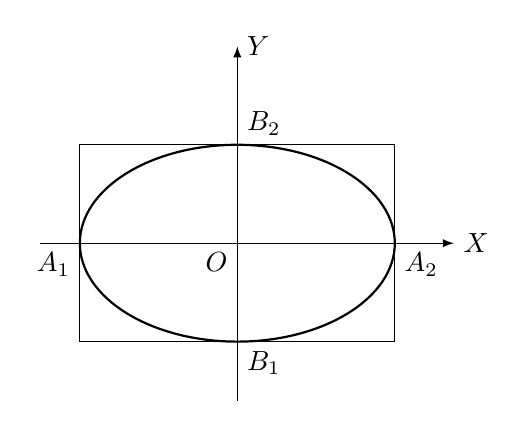
\begin{tikzpicture}[>=latex]
\draw[->](-2.5,0)--(2.75,0)node[right]{$X$};
\draw[->](0,-2)--(0,2.5)node[right]{$Y$};
\draw[thick](0,0) ellipse [x radius=2, y radius=1.25];        
\node at (0,0)[below left]{$O$};
\draw(-2,-1.25) rectangle (2,1.25);
\node at (-2,0)[below left]{$A_1$};
\node at (2,0)[below right]{$A_2$};
\node at (0,1.25)[above right]{$B_2$};
\node at (0,-1.25)[below right]{$B_1$};
\tkzDrawPoint(1.5,0)\tkzDrawPoint(-1.5,0)
    \end{tikzpicture}
    \caption{}
\end{figure}

当$y=0$, $x=\pm a$, 点$A_1(-a,0)$, $A_2(+a,0)$
是$X$轴上距$Y$轴最远的两个点,当$x=0$, $y=\pm b$, 点
$B_1(0,-b)$, $B_2(0,+b)$是$Y$轴上距$X$轴距离最远的
两个点,这四点,$A_1$、$A_2$、$B_1$、$B_2$叫做\textbf{椭圆的顶点}.
$\overline{A_1A_2},\overline{B_1B_2}$分别叫做椭圆的长和轴短轴.$\overline{A_1A_2}=2a$, 
$\overline{B_1B_2}=2b$, $a$和$b$分别叫做椭圆的\textbf{长半轴长和短半轴长}.
长轴和短轴的交点叫做\textbf{椭圆的中心}.

如果$a=b$, 那么方程(6.2)化为
\[x^2+y^2=a^2\]
这时椭圆成为圆,$c=\sqrt{a^2-b^2}=0$, 即椭圆的两个焦点重
合于圆心,因此可以说\textbf{圆是椭圆的特殊情形}.

由以上讨论可以看出,椭圆的形状依赖于$a$和$b$, 数量
$c=\sqrt{a^2-b^2}$可表示出椭圆离开圆的偏差.由$c^2=a^2-b^2$
可得
\[\frac{c}{a}=\sqrt{1-\left(\frac{b}{a}\right)^2},\qquad \frac{b}{a}=\sqrt{1-\left(\frac{c}{a}\right)^2}\]
比值
\[e=\frac{c}{a}=\frac{\sqrt{a^2-b^2}}{a}\]
叫做\textbf{椭圆的离心率},用它可同样来表出椭圆的形状.由$c<
a$, 可知$e<1$, 当离心率愈来愈大时,也就是愈来愈接近
1时,$1-e^2$就越小,椭圆的形状就愈扁平;反之,就愈接
近于圆,当$e=0$时,$a=b$椭圆就成为圆了.

如果椭圆的中心在原点,焦点在$Y$轴上,那么长轴也-
定在$Y$轴上,这时两个焦点$F_1,F_2$的坐标分别是$(0,-c)$,
$(0,c)$ (图6.3), 求得圆的标准方程是
\begin{equation}
    \boxed{\frac{x^2}{b^2}+\frac{y^2}{a^2}=1}\qquad a\ge b>0
\end{equation}
把方程(6.2)的变量$x$和$y$互换就可得到方程(6.6).

\begin{figure}[htp]\centering
    \centering
\begin{tikzpicture}[>=latex, scale=1]
    \draw[->](-1.5,0)--(1.75,0)node[right]{$X$};
    \draw[->](0,-2)--(0,2.5)node[right]{$Y$};
    \draw[thick](0,0) ellipse [x radius=.7, y radius=1.5];  
    \tkzDefPoints{0/-1.2/F_1, 0/1.2/F_2}
\tkzLabelPoints[right](F_1,F_2)
\tkzDrawPoints(F_1,F_2)
\node at (0,0)[below left]{$O$}; 
\node at (0,1.5)[above right]{$B(0,a)$}; 
\node at (0.7,0)[below right]{$A(b,0)$}; 
    \end{tikzpicture}
    \caption{}
    \end{figure}


\begin{example}
    已知椭圆的长轴长是10, 焦距是8, 求椭圆的标准方程.
\end{example}

\begin{solution}
    由已知条件得$2a=10,\quad 2c=8$,所以:
\[a=5,\qquad c=4,\qquad b^2=a^2-c^2=5^2-4^2=9\]
因此所求椭圆的标准方程为
\[\frac{x^2}{25}+\frac{y^2}{9}=1\]
\end{solution}

\begin{example}
    求椭圆$4x^2+9y^2=36$的长轴、短轴长、离心率、
焦点和顶点的坐标,并用描点法画出它的图形.
\end{example}

\begin{solution}
    已知方程可化为
    \[\frac{x^2}{9}+\frac{y^2}{4}=1\]
这是长轴在$X$轴上,中心在坐标原点的椭圆标准方程.
因此$a=3$, $b=2$, $c=\sqrt{3^2-2^2}=\sqrt{5}$, 顶点$A'(-3,
0)$, $A(3,0)$, $B'(0,-2)$, $B(0,2)$. 焦点
$F_1(-\sqrt{5},0)$, $F_2(\sqrt{5},0)$. 离心率$e=\frac{c}{a}=\frac{\sqrt{5}}{3}$.

在第I象限已知椭圆方程可写为
\[y=\frac{2}{3}\sqrt{9-x^2},\qquad 0\le x\le 3\]
算出一些满足所求椭圆方程的点的坐标$(x,y)$:
\begin{center}
    \begin{tabular}{cccccccc}
\hline
$x$&0&0.5&1&1.5&2&2.5&3\\
\hline
$y$&2&1.97&1.89&1.73&1.49&1.11&0\\
\hline
    \end{tabular}
\end{center}
描点画出椭圆在第I象限的图
象,然后根据椭圆的对称性就可
画出整个椭圆的图象(图6.4).
\end{solution}

\begin{figure}[htp]\centering
    \begin{minipage}[t]{0.48\textwidth}
    \centering
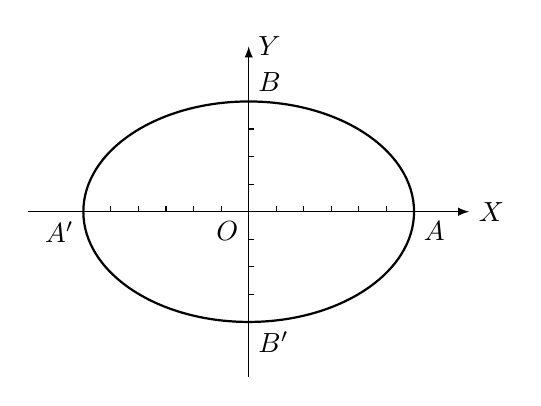
\begin{tikzpicture}[>=latex, scale=.7]
    \draw[->](-4,0)--(4,0)node[right]{$X$};
    \draw[->](0,-3)--(0,3)node[right]{$Y$};
    \draw[thick](0,0)node[below left]{$O$} ellipse [x radius=3, y radius=2];  
    \node at (-3,0)[below left]{$A'$};
    \node at (3,0)[below right]{$A$};
    \node at (0,2)[above right]{$B$};
    \node at (0,-2)[below right]{$B'$};
\tkzDefPoints{0/2/A, .5/1.97/B, 1/1.89/C, 1.5/1.73/D, 2/1.49/E, 2.5/1.11/F, 3/0/G}
\tkzDrawPoints(A,B,C,D,E,F,G)

\tkzDefPoints{0/-2/A, .5/-1.97/B, 1/-1.89/C, 1.5/-1.73/D, 2/-1.49/E, 2.5/-1.11/F, 3/0/G}
\tkzDrawPoints(A,B,C,D,E,F,G)

\tkzDefPoints{0/2/A, -.5/1.97/B, -1/1.89/C, -1.5/1.73/D, -2/1.49/E, -2.5/1.11/F, -3/0/G}
\tkzDrawPoints(A,B,C,D,E,F,G)

\tkzDefPoints{0/-2/A, -.5/-1.97/B, -1/-1.89/C, -1.5/-1.73/D, -2/-1.49/E, -2.5/-1.11/F, -3/0/G}
\tkzDrawPoints(A,B,C,D,E,F,G)

\foreach \x in {-2.5,-2,...,2.5}
{
    \draw(\x,0)--(\x,.1);
}
\foreach \x in {-1.5,-1,...,1.5}
{
    \draw(0,\x)--(.1,\x);
}
    \end{tikzpicture}
    \caption{}
    \end{minipage}
    \begin{minipage}[t]{0.48\textwidth}
    \centering
    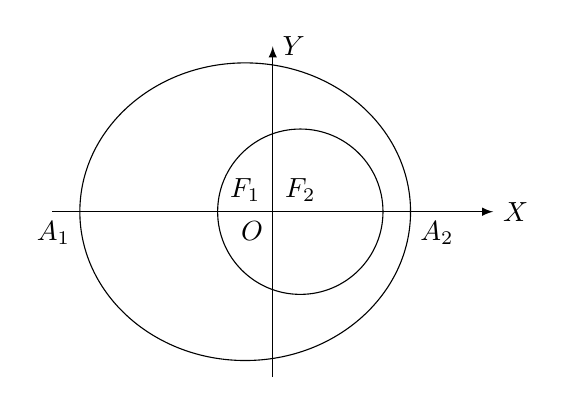
\begin{tikzpicture}[>=latex, scale=.7]
        \draw[->](-4,0)--(4,0)node[right]{$X$};
        \draw[->](0,-3)--(0,3)node[right]{$Y$};
    \draw(.5,0)node[above]{$F_2$} circle(1.5);
    \draw(-.5,0)node[above]{$F_1$} ellipse[x radius= 3,  y radius= 2.7];
    \tkzDrawPoint(.5,0)\tkzDrawPoint(-.5,0)
    \node at (0,0) [below left]{$O$};
    \node at (2.5,0) [below right]{$A_2$};
    \node at (-3.5,0) [below left]{$A_1$};
    \end{tikzpicture}
    \caption{}
    \end{minipage}
    \end{figure}


\begin{example}
    我国第一颗人造地球
卫星的运行轨道是以地球中心为
一焦点的椭圆,卫星的近地点与
地球表面距离为439公里;远地点
与地球表面距离为2384公里,已知地球半径约为6371公里,
试求卫星轨道的近似方程及其离心率.
\end{example}


\begin{solution}
    设地球中心$F_2$在$X$轴上(图6.5),所求方程为
\[\frac{x^2}{a^2}+\frac{y^2}{b^2}=1\]
依题意
\[\begin{split}
    \overline{A_1F_2}&=a+c=6371+2284=8755\\
    \overline{A_2F_2}&=a-c=6371+439=6810
\end{split}\]
由以上两式联立求解得
\[a=7782.5,\qquad c=972.5,\qquad b=\sqrt{a^2-c^2}=7721.5\]
所以,所求卫星轨道的近似方程为
\[\frac{x^2}{(7782.5)^2}+\frac{y^2}{(7721.5)^2}=1\]
其离心率
$e=\frac{c}{a}\approx 0.125$
\end{solution}

\begin{ex}
\begin{enumerate}
    \item 已知椭圆的长轴长是6, 短轴长是2, 焦点在$X$轴上,
    求这椭圆的标准方程并画出这椭圆的草图.
    \item 在第1题中,若焦点在$Y$轴,椭圆的标准方程为何?
    \item 已知椭圆的一个焦点是$F_1(-3,0)$与$X$轴一个交点
    $A(4,0)$, 求此椭圆的方程.
    \item 求以下椭圆的长轴长,短轴长、焦点的坐标及其离心率.
\begin{multicols}{2}
\begin{enumerate}
    \item $\frac{x^2}{100}+\frac{y^2}{36}=1$
    \item $25x^2+9y^2=100$
    \item $\frac{x^2}{16}+\frac{y^2}{64}=1$
    \item $49x^2+9y^2=2500$
\end{enumerate}
\end{multicols}

\item 已知椭圆中心在原点,一焦点是$F(3,0)$, 椭圆与$X$
轴相交于$A$、$A'$两点,$\overline{AF}=2$, $\overline{A'F}=8$, 求此椭圆的方程.
\item 已知地球的轨道是一个椭圆,太阳在它的一个焦点上,
长轴长约30亿公里,离心率$e=1/60$, 
求地球的轨道方程,地球的轨道中心与太阳的距离,以及近日点,远日
点到太阳的距离.
\item 试求平分圆$x^2+y^2=25$上各点的纵坐标,而横坐标不
变的点的轨迹方程.
\item 试求把圆$x^2+y^2=100$上各纵坐标分为2:3, 而横
坐标不变的点的轨迹方程.
\item 一动点与直线$x=8$的距离是它与点$(2,0)$的距离的
2倍,求这动点的轨迹方程.
\item 一定长为$a$的线段,两端在互相垂直的二直线上移动,
试求此线段上任意一点的轨迹方程.
\item 设一三角形的一边的两个端点为$(0,6)$, $(0,-6)$,其它两
边斜率的乘积是$-\frac{4}{9}$,
试求另一顶点的轨迹.
\item 已知$A>0$, $B>0$, 且$A<B$, 试求椭圆$Ax^2+By^2
=C$的焦点坐标.
\item 试证:椭圆的短半轴长是其中一焦点到长轴两顶点距离
的比例中项.
\item 在椭圆$\frac{x^2}{45}+\frac{y^2}{20}=1$上求一点,使它与两焦点连线互相垂直.
\end{enumerate}
\end{ex}

\subsection{双曲线的标准方程和形状}
\begin{blk}
    {定义} 平面内到两定点距离的差的绝对值等于常数(常
数小于两定点间的距离)的轨迹叫做双曲线.这两个定点叫
做双曲线的焦点,两个焦点间的距离叫做焦距.
\end{blk}

根据双曲线的定义,我们来求它的方程:
\begin{figure}[htp]
    \centering
\begin{tikzpicture}[>=latex, yscale=.7]
\draw[->](-2.5,0)--(2.5,0)node[right]{$X$};
\draw[->](0,-2.5)--(0,2.5)node[right]{$Y$};    
\draw[domain=-2:2, samples=100, very thick]plot({sqrt(1+\x*\x)}, \x);
\draw[domain=-2:2, samples=100, very thick]plot({-sqrt(1+\x*\x)}, \x);
\tkzDefPoints{-1.414/0/F_1, 1.414/0/F_2, 2/1.732/P}
\tkzDrawSegments[thick](F_1,P F_2,P)
\tkzLabelPoints[below](F_1, F_2)
\tkzLabelPoints[above](P)
\node at (0,0)[below left]{$O$};
\end{tikzpicture}
    \caption{}
\end{figure}

设$F_1$、$F_2$是双曲线的两个焦点,取射线$F_1F_2$的方向作
为$X$轴的正方向,$\overline{F_1F_2}$的垂直平分线作为$Y$轴(图6.6).
若$\overline{F_1F_2}=2c$, 则两焦点的坐标分别为$F_1(-c,0)$, $F_2
(c,0)$. 

再设$P(x,y)$是双曲线上任一点,则由双曲线的定义
有
\[|\overline{PF_1}-\overline{PF_2}|=2a\]
因$\overline{PF_1}=\sqrt{(x+c)^2+y^2}$, $\overline{PF_2}=
\sqrt{(x-c)^2+y^2}$, 
代入上式,得方程
\[\sqrt{(x+c)^2+y^2}-\sqrt{(x-c)^2+y^2}=\pm 2a\]
去根号,整理得
\begin{equation*}
    (a^2-c^2)x^2+a^2y^2=a^2(a^2-c^2)
\end{equation*}
这个式子和上节得到的椭圆方程(6.1)在外形上完全一样,
这里,由双曲线的定义$2c>2a$, 即
\[c>a\]
所以$a^2-c^2<0$, 故设$a^2-c^2=-b^2\; (b>0)$, 代入(6.1)
式得
\[-b^2x^2+a^2y^2=-a^2b^2\]
两边同除$-a^2b^2$得
\begin{equation}
    \boxed{\frac{x^2}{a^2}-\frac{y^2}{b^2}=1}
\end{equation}

由上述推导过程说明,凡在双曲线上的点,它的坐标一
定满足方程(6.5); 反过来,
设$P_1(x_1,y_1)$的坐标满足方程(6.5), 则
\[\begin{split}
    \frac{x^2_1}{a^2}-\frac{y^2_1}{b^2}&=1\\
    \overline{P_1F_1}&=\sqrt{(x_1+c)^2+y_1^2}
\end{split}\]
但
\[y^2_1=b^2\left(\frac{x_1^2}{a^2}-1\right)=(c^2-a^2)\left(\frac{x_1^2}{a^2}-1\right)\]
代入上式,化简可得
\begin{equation}
    \overline{P_1F_1}=\left|\frac{c}{a}x_1+a\right|
\end{equation}
同理可求
\begin{equation}
    \overline{P_1F_2}=\left|\frac{c}{a}x_1-a\right|
\end{equation}

因为$c>a$, $|x|\ge a$, 所以$\left|\frac{c}{a}x_1\right|>a$,
$\frac{c}{a}x_1+a$及$\frac{c}{a}x_1-a$与$\frac{c}{a}x_1$同号.

当$x_1>0$时
\[\overline{P_1F_1}=\frac{c}{a}x_1+a,\qquad \overline{P_1F_2}=\frac{c}{a}x_1-a\]
因此,
\[\overline{P_1F_1}-\overline{P_1F_2}=2a\]

当$x_1<0$时,
\[\overline{P_1F_1}=-\left(\frac{c}{a}x_1+a\right),\qquad \overline{P_1F_2}=-\left(\frac{c}{a}x_1-a\right)\]
因此,
\[\overline{P_1F_1}-\overline{P_1F_2}=-2a\]

这就证明了,凡坐标适合方程(6.5)的点都在双曲线
上,由以上证明,所以方程(6.5)是所求的双曲线的方程,
并且我们把方程(6.5)叫做\textbf{双曲线的标准方程},它所表示的
双曲线的焦点在$X$轴上,焦点是$F_1(-c,0)$、$F_2(c,0)$.
这里$c^2=a^2+b^2$.

如果取$F_1$、$F_2$的连线作为$Y$轴,取$F_1F_2$的垂直平分
线作为$X$轴,在这一坐标系中,仿上面的方法可得双曲线的
方程为
\begin{equation}
    \boxed{\frac{y^2}{a^2}-\frac{x^2}{b^2}=1}
\end{equation}
只要将方程(6.5)中的$x$与$y$对调就可得到方程(6.8), 这一
方程也叫做双曲线的标准方程,它表示双曲线的焦点在$Y$轴
上,焦点是$F_1(0,-c)$, $F_2(0,c)$, $c^2=a^2+b^2$.

下面我们用双曲线的标准方程研究它的几何形状.

首先,与椭圆方程一样,方程(6.5)中只含有$x$、$y$的
平方,故把其中一个坐标变号,对于方程没有影响,这就表
明,如果点$M(x,y)$在双曲线上,那么$M_1(x,-y)$、$M_2(-x,
-y)$、$M_3(-x,y)$等也都在双曲线上,所以,双曲线是以
$X$轴或$Y$轴为对称轴的轴对称图形,又是以坐标原点为对称
中心的中心对称图形,对称中心又叫做双曲线的中心,其
次,由方程(6.5)得
\[\frac{x^2}{a^2}\ge 1,\qquad x^2\ge a^2\]
则$x\ge a$或$x\le -a$.这说明双曲线在两条直线$x=a$, $x=-a$所夹平面区域的外侧,最后我们讨论双曲线在第I象限内的性态,在第I象
限,方程(6.5)可写为
\[y=\frac{b}{a}\sqrt{x^2-a^2}\qquad (x\ge a)\]

\begin{figure}[htp]
    \centering
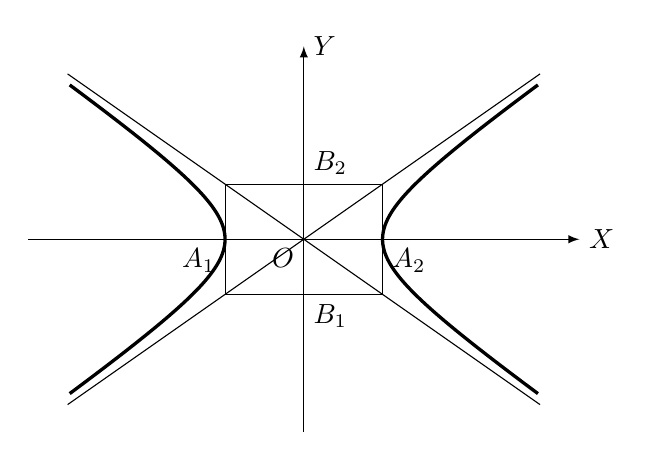
\begin{tikzpicture}[>=latex, yscale=.7]
\draw[->](-3.5,0)--(3.5,0)node[right]{$X$};
\draw[->](0,-3.5)--(0,3.5)node[right]{$Y$};    
\draw[domain=-2.8:2.8, samples=100, very thick]plot({sqrt(1+\x*\x)}, \x);
\draw[domain=-2.8:2.8, samples=100, very thick]plot({-sqrt(1+\x*\x)}, \x);
\draw(-3,3)--(3,-3);
\draw(3,3)--(-3,-3);
\draw(-1,-1) rectangle (1,1);
\node at (0,0)[below left]{$O$};
\node at (-1,0)[below left]{$A_1$};
\node at (1,0)[below right]{$A_2$};
\node at (0,1)[above right]{$B_2$};
\node at (0,-1)[below right]{$B_1$};
\end{tikzpicture}
    \caption{}
\end{figure}

当$x=a$时,$y=0$, 当$x$由$a$递增且趋向$\infty$, $y$也由0递
增趋向,方程的轨迹趋向无穷远(图6.7),但由于
\[y=\frac{b}{a}\sqrt{x^2-a^2}=\frac{b}{a}x\sqrt{1-\left(\frac{a}{x}\right)^2}<\frac{b}{a}x\]
即
\[\frac{b}{a}x-\frac{b}{a}\sqrt{x^2-a^2}>0\]
所以,当$x$由$a$趋向$\infty$时,相应的$y$值愈来愈接近$\frac{b}{a}x$, 而
又不会大于$\frac{b}{a}x$,
这说明,双曲线在第I象限的部分永远在
射线$y=\frac{b}{a}x\; (x\ge 0)$的下方并且逐渐接近于射线$y=\frac{b}{a}x\; (x\ge 0)$. 由对称性,可推知双曲线在其它象限的性态
(图6.7).

直线$y=\frac{b}{a}x$和$y=-\frac{b}{a}x$叫做\textbf{双曲线的渐近线}.

令$y=0$, $x=\pm a$, 点$A_1(-a,0)$, $A_2(a,0)$叫
做双曲线的顶点,$\overline{A_1A_2}$叫做双曲线的\textbf{实轴},它的长等于
$2a$, $a$叫做双曲线的实半轴长.

令$x=0$, $y=\pm b\sqrt{-1}$, 这说明双曲线和$Y$轴没有
交点.在$Y$轴上作$B_1(0,-b)$, $B_2(0,b)$, $\overline{B_1B_2}$叫做双
曲线的虚轴,它的长等于$2b$, $b$叫做双曲线虚半轴长(图6
.7).实轴和虚轴等长的双曲线叫做\textbf{等轴双曲线}.

以已知双曲线的虚轴为实轴,实轴为虚轴所得到的双曲
线叫做原双曲线的\textbf{共轭双曲线}.由这个定义可知,双曲线
$\frac{x^2}{a^2}-\frac{y^2}{b^2}=1$与$\frac{x^2}{a^2}-\frac{y^2}{b^2}=-1$
是互为共轭双曲线(图6.8).

作为练习,请同学证明:双曲线和它的共轭双曲线有相
词的渐近线.

\begin{figure}[htp]
    \centering
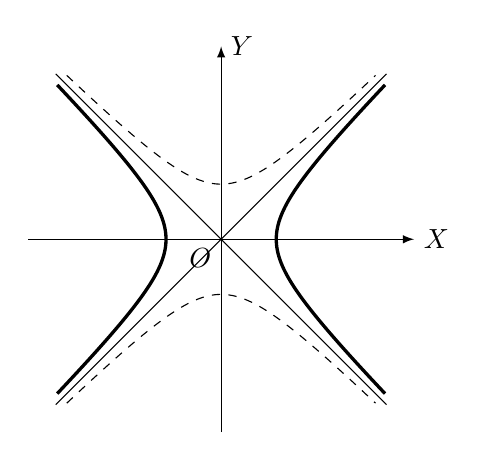
\begin{tikzpicture}[>=latex, scale=.7]
 \draw[->](-3.5,0)--(3.5,0)node[right]{$X$};
\draw[->](0,-3.5)--(0,3.5)node[right]{$Y$};    
\node at (0,0)[below left]{$O$};
\draw[domain=-2.8:2.8, samples=100, very thick]plot({sqrt(1+\x*\x)}, \x);
\draw[domain=-2.8:2.8, samples=100, very thick]plot({-sqrt(1+\x*\x)}, \x);
\draw(-3,3)--(3,-3);
\draw(3,3)--(-3,-3);
\draw[domain=-2.8:2.8, samples=100, dashed]plot(\x, {sqrt(1+\x*\x)});
\draw[domain=-2.8:2.8, samples=100, dashed]plot( \x, {-sqrt(1+\x*\x)});


\end{tikzpicture}
    \caption{}
\end{figure}

和定义椭圆的离心率$e$一样,对于双曲线,比值
\[e=\frac{c}{a}=\frac{\sqrt{a^2+b^2}}{a}=\sqrt{1+\left(\frac{b}{a}\right)^2}\]
也叫做双曲线的离心率,因为$c>a$, 所以双曲线的离心率
$e>1$, 容易看出,$\frac{b}{a}$越大,$e$越大;反之,$e$越大,
$\frac{b}{a}$也越大,渐近线$y=\pm \frac{b}{a}x$的斜率的绝对值也越大,这时双曲
线的开口增大越快.


\begin{example}
    设双曲线两焦点间的距离等于8, 顶点间的距离
等于6, 实轴在$X$轴上,求双曲线的标准方程,离心率,渐
近线方程并画草图.
\end{example}

\begin{solution}
    依题意$2c=8$, $2a=6$, 所以$c=4$, $a=3$,
\[    b^2=c^2-a^2=16-9=7,\qquad  b=\sqrt{7}\]
    所求双曲线方程为
\[\frac{x^2}{9}-\frac{y^2}{7}=1\]
离心率$e=\frac{c}{a}=\frac{4}{3}$,渐近线方程为
\[y=\frac{\sqrt{7}}{3}x,\qquad y=-\frac{\sqrt{7}}{3}x\]

作图:如图6.9所示
\begin{enumerate}
\item 在$X$轴上作$A_1(-3,
0)$, $A_2(3,0)$, 在$Y$轴上作$B_1(0,-\sqrt{7})$、$B_2(0,
\sqrt{7})$, 过$A_1$、$A_2$、$B_1$、$B_2$作矩形$ABCD$, 直线$OA$, 
$OB$为双曲线的渐近线.
\item 算出一些满足所求双曲线方程的点的坐标:
\begin{center}
\begin{tabular}{ccccc}
\hline
$x$ & $\pm 4$ & $\pm 5$ & $\pm 6$ & $\pm 7$\\
\hline
$y$ &  $\pm 2.3$ & $\pm 3.5$ & $\pm 4.6$ & $\pm 5.6$\\
\hline
\end{tabular}
\end{center}
描点连线,使曲线与渐近线逐渐接近,就可得到双曲线的草图.
\end{enumerate}
\end{solution}


\begin{figure}[htp]
    \centering
\begin{tikzpicture}[>=latex, scale=.4]
 \draw[->](-8.5,0)--(8.5,0)node[right]{$X$};
\draw[->](0,-8.5)--(0,8.5)node[right]{$Y$};    
\node at (0,0)[below left]{$O$};

\draw[domain=-7:7, samples=100, very thick]plot({sqrt(9+9/7*\x*\x)}, \x);
\draw[domain=-7:7, samples=100, very thick]plot({-sqrt(9+9/7*\x*\x)}, \x);
\draw(-3*3,2.65*3)--(3*3,-2.65*3);
\draw(3*3,2.65*3)--(-3*3,-2.65*3);
\draw(-3,-2.65) rectangle(3,2.65);

\tkzDefPoints{-3/-2.65/C, 3/-2.65/D, -3/2.65/B, 3/2.65/A}
\tkzDefPoints{-3/0/A_1, 3/0/A_2, 0/2.65/B_2, 0/-2.65/B_1}
\tkzLabelPoints[above](A,B)
\tkzLabelPoints[below](C,D)
\tkzLabelPoints[above left](B_2)
\tkzLabelPoints[below left](B_1)
\tkzLabelPoints[below left](A_2)
\tkzLabelPoints[below right](A_1)

\tkzDefPoints{4/0/F_2, -4/0/F_1}
\tkzLabelPoints[below](F_1,F_2)
\tkzDrawPoints(F_1,F_2,A_1,A_2,B_1,B_2)

\tkzDefPoints{4/2.3/A1, 5/3.5/A2, 6/4.6/A3, 7/5.6/A4}
\tkzDrawPoints(A1,A2,A3,A4)
\tkzDefPoints{4/-2.3/A1, 5/-3.5/A2, 6/-4.6/A3, 7/-5.6/A4}
\tkzDrawPoints(A1,A2,A3,A4)
\tkzDefPoints{-4/2.3/A1, -5/3.5/A2, -6/4.6/A3, -7/5.6/A4}
\tkzDrawPoints(A1,A2,A3,A4)
\tkzDefPoints{-4/-2.3/A1, -5/-3.5/A2, -6/-4.6/A3, -7/-5.6/A4}
\tkzDrawPoints(A1,A2,A3,A4)

\foreach \x in {-7,-6,...,7}
{
    \draw(\x,0)--(\x,.2);
    \draw(0,\x)--(.2,\x);
}
\end{tikzpicture}
    \caption{}
\end{figure}



\begin{example}
    证明:双曲线上任一点到两条渐近线的距离的乘积等于常数$\frac{a^2b^2}{a^2+b^2}$
\end{example}

\begin{proof}
    已知双曲线$\frac{x^2}{a^2}-\frac{y^2}{b^2}=1$,它的两条渐近线方程为
\[\ell_1:\; bx+ay=0,\qquad \ell_2:\; bx-ay=0\]
设$P(x_1,y_1)$为双曲线上任一点,$P$到$\ell_1$的距离记为$d_1$,$P$
到$\ell_2$的距离记为$d_2$,则:
\[d_1=\frac{|bx_1+ay_1|}{\sqrt{a^2+b^2}},\qquad d_2=\frac{|bx_1-ay_1|}{\sqrt{a^2+b^2}}\]
\[d_1\cdot d_2=\frac{|bx_1+ay_1|}{\sqrt{a^2+b^2}}\cdot \frac{|bx_1-ay_1|}{\sqrt{a^2+b^2}}=\frac{|b^2x^2_1-a^2y^2_1|}{{a^2+b^2}}\]
但
\[|b^2x^2_1-a^2y^2_1|=a^2b^2\]
所以
\[d_1\cdot d_2=\frac{a^2b^2}{a^2+b^2}\]    
\end{proof}

\begin{ex}
\begin{enumerate}
    \item 求适合下列条件的双曲线的标准方程.
\begin{enumerate}
\item 实轴长为12, 虚轴长为$2\sqrt{13}$, 
    焦点在$X$轴上;
    \item 实轴长为5, 虚轴长为3, 焦点在$Y$轴上;
    \item 焦距是10, 两顶点间的距离是8; 
    实轴在$X$轴上;
    \item 实轴长等于4, 且经过点$A(2,4)$, 实轴在$X$
    轴上;
    \item 实轴长等于4, 且经过点$A(2,4)$, 实轴在$Y$轴
    上.
\end{enumerate}
\item 求下列双曲线的实轴和虚轴长,顶点和焦点的坐标,离
心率和渐近线方程.
\begin{multicols}{2}
\begin{enumerate}
    \item $x^2-y^2=1$
    \item $\frac{x^2}{5}-\frac{y^2}{9}=1$
    \item $4x^2-y^2=16$
    \item $x^2-y^2=-1$
    \item $\frac{x^2}{25}-y^2=-1$
\end{enumerate}
\end{multicols}

\item 画出双曲线$\frac{x^2}{16}-\frac{y^2}{9}=1$的草图.
\item 等轴双曲线的一个焦点$F_1(-4,0)$, 求它的标准方
程.
\item 证明:
\begin{enumerate}
\item 双曲线和它的共轭双曲线有共同的渐近
线;
\item 双曲线和它的共轭双曲线的四个焦点在同一个圆
上.
\end{enumerate}

\item 已知双曲线
$\frac{x^2}{9}-\frac{y^2}{16}=1$, 求出它的共领双曲线方程并
求共轭双曲线的焦点的坐标,渐近线方程和离心率.
\end{enumerate}
\end{ex}

\subsection{抛物线的标准方程和形状}
\begin{blk}
   {定义}
平面内与一定点和一条定直线的距离相等的点的轨迹叫做抛物线.定点叫做抛物线的焦点,定直线叫做抛物
线的准线.
\end{blk}

下面,我们根据抛物线的定义来建立抛物线的方程.

\begin{figure}[htp]
    \centering
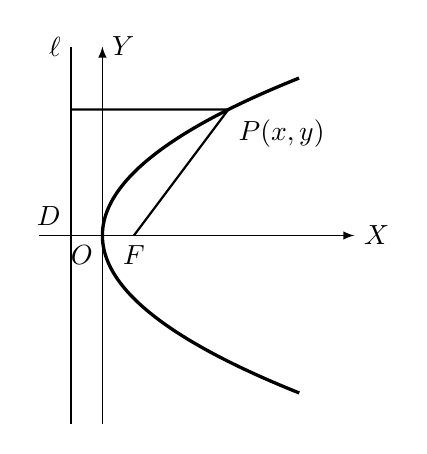
\begin{tikzpicture}[>=latex, scale=.8]
 \draw[->](-1,0)--(4,0)node[right]{$X$};
\draw[->](0,-3)--(0,3)node[right]{$Y$};
\draw[thick](-.5,-3)--(-.5,0)node[above left]{$D$}--(-.5,3)node[left]{$\ell$};
\draw[domain=-2.5:2.5, samples=100, very thick]plot({0.5*\x*\x}, \x);
\draw[thick](-.5,2)--(2,2)node[below right]{$P(x,y)$}--(.5,0)node[below]{$F$};
\node at (0,0)[below left]{$O$};
\end{tikzpicture}
    \caption{}
\end{figure}

设焦点为$F$, 准线为$\ell$ (图
6.10),过$F$点作$\ell$的垂线与$\ell$相交于$D$点,取射线$DF$的方向
作为$X$轴的正方向,以$\overline{DF}$的垂直平分线为$Y$轴,设$F$到$\ell$的距离为$p$, 即$\overline{DF}=p$, 则
\[F\left(\frac{p}{2},0\right),\qquad D\left(-\frac{p}{2},0\right)\]
准线$\ell$的方程为
\[x=-\frac{p}{2}\]

设$P(x,y)$是抛物线上任一点,它到焦点$F$的距离等
于它到$\ell$的距离.即
\[\sqrt{\left(x-\frac{p}{2}\right)^2+y^2}=\left|x+\frac{p}{2}\right|\]
将上式两边平方,并化简得
\begin{equation}
    y^2=2px\qquad (p>0)
\end{equation}
这就是说,凡是在抛物线上的点,它的坐标都适合这一方
程;反过来,设$P(x_1,y_1)$的坐标满足方程(6.9), 则
$y_1^2=2px_1$. 点$P(x_1,y_1)$与焦点$F$的距离
\[\begin{split}
    PF=\sqrt{\left(x_1-\frac{p}{2}\right)^2+y^2_1}&=\sqrt{\left(x_1-\frac{p}{2}\right)^2+2px_1}\\
    &=\sqrt{\left(x_1+\frac{p}{2}\right)^2}=\left|x_1+\frac{p}{2}\right|
\end{split}\]
这就是点$P$到准线的距离,这就证明了,凡坐标适合方程(6.9)
的点,都在抛物线上.

由以上证明,所以方程(6.9)是所求的抛物线方程,并
把方程(6.9)叫做\textbf{抛物线的标准方程}.它表示的抛物线的焦
点$F$在$X$轴的正半轴上且坐标是$\left(\frac{p}{2},0\right)$
准线方程是$x=-\frac{p}{2}$.

如果抛物线的焦点和准线分别取
\[\begin{split}
F\left(-\frac{p}{2},0\right),\quad x=\frac{p}{2}&\qquad \text{(图6.11)}\\
F\left(0,\frac{p}{2}\right),\quad y=-\frac{p}{2}&\qquad \text{(图6.12)}\\
F\left(-\frac{p}{2},0\right),\quad y=\frac{p}{2}&\qquad \text{(图6.13)}\\
\end{split}\]
可分别类似地得到抛物线标准方程为
\[y^2=-2px,\qquad x^2=2py,\qquad x^2=-2py\]

\begin{figure}[htp]\centering
    \begin{minipage}[t]{0.3\textwidth}
    \centering
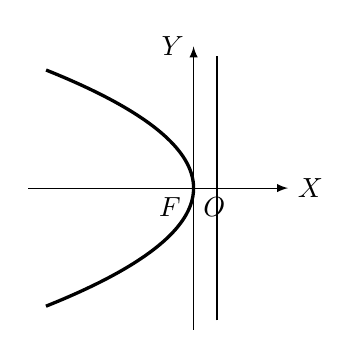
\begin{tikzpicture}[>=latex, scale=.6]
\draw[->](-3.5,0)--(2,0)node[right]{$X$};
\draw[->](0,-3)--(0,3)node[left]{$Y$};
\draw[thick](.5,-2.8)--(.5,2.8);
\draw[domain=-2.5:2.5, samples=100, very thick]plot({-0.5*\x*\x}, \x);
\node at (-.5,0) [below]{$F$};
\tkzDrawPoint (-.5,0) 
\node at (0,0)[below right]{$O$};
    \end{tikzpicture}
    \caption{}
    \end{minipage}
    \begin{minipage}[t]{0.3\textwidth}
    \centering
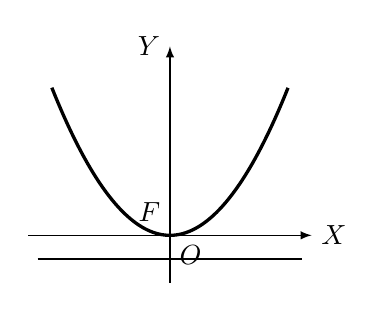
\begin{tikzpicture}[>=latex, scale=.6]
\draw[->](-3,0)--(3,0)node[right]{$X$};
\draw[->](0,-1)--(0,4)node[left]{$Y$};
\draw[thick](-2.8,-.5)--(2.8,-.5);
\draw[domain=-2.5:2.5, samples=100, very thick]plot(\x,{0.5*\x*\x});
\node at (0,.5) [left]{$F$};
\tkzDrawPoint (0,.5) 
\node at (0,0)[below right]{$O$};
    \end{tikzpicture}
    \caption{}
    \end{minipage}
    \begin{minipage}[t]{0.3\textwidth}
    \centering
    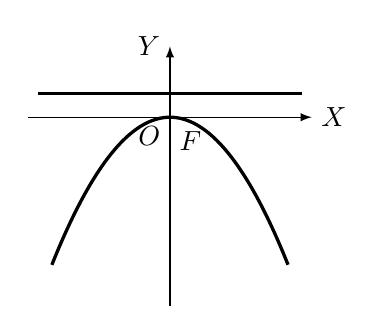
\begin{tikzpicture}[>=latex, scale=.6]
\draw[->](-3,0)--(3,0)node[right]{$X$};
\draw[->](0,-4)--(0,1.5)node[left]{$Y$};
\draw[thick](-2.8,.5)--(2.8,.5);
\draw[domain=-2.5:2.5, samples=100, very thick]plot(\x,{-0.5*\x*\x});
\node at (0,-.5) [right]{$F$};
\tkzDrawPoint (0,-.5) 
\node at (0,0)[below left]{$O$}; 
    \end{tikzpicture}
    \caption{}
    \end{minipage}
    \end{figure}

下面我们用抛物线的标准方程来研究抛物线的形状.

首先,在方程(6.9)中,含有$y$的平方,故把$-y$代替$y$对
方程没有影响,这表明曲线是\textbf{以$X$轴为对称轴的轴对称形}.
我们把这条轴叫做\textbf{抛物线的轴}.轴和抛物线的交点叫做\textbf{抛物
线的顶点}.

其次,由方程(6.9)可知$x\ge 0$, 当$x$增大时,$y$的绝
对值也跟着增大,因此抛物线在$Y$轴的右方,向上、向下无
限伸展.设$P(x,y)$是抛物线上任一点,直线$OP$的倾角为
$\alpha$, 则
\[\tan\alpha=\frac{y}{x}=\frac{y^2}{xy}=\frac{2px}{xy}=\frac{2p}{y}\]
其中$p$是常数,当$y$无限增大时,$\frac{2p}{y}$
无限接近于零,这说
明,抛物线上动点$P(x,y)$无限远离原点时,$P(x,y)$点
到$X$轴的距离无限增大,而$\Vec{OP}$的方向与$X$轴正向之间的方
向差却趋于零,这是抛物线与双曲线的重要区别之一.

\begin{example}
    已知抛物线的焦点$F(2,0)$, 求它的标准方
程.
\end{example}


\begin{solution}
    因为焦点$F(2,0)$在$X$轴上,
$\frac{p}{2}=2$, $p=4$, 
所以抛物线标准方程是
\[y^2=8x\]
\end{solution}



\begin{example}
    已知抛物线的标准方程是$y^2=-4x$, 求它的焦点
坐标和准线方程.
\end{example}

\begin{solution}
    因为$p=-2$, 所以焦点的坐标是$(-1,0)$, 
准线方程是$x=1$.
\end{solution}

\begin{ex}
\begin{enumerate}
    \item 根据下列抛物线方程,求出焦点的坐标,准线方程,并
    画出草图.
\begin{multicols}{2}
\begin{enumerate}
  \item $y^2=10x$  
\item $y^2=-10x$
\item $x^2=12y$  
\item $y^2=-8x$
\end{enumerate}
\end{multicols}

    \item 证明:抛物线$y^2=2px$纵坐标中点的轨迹方程,是
$y^2=\frac{p}{2}x$
    \item 由下列已知条件,求抛物线的标准方程.
\begin{enumerate}
\item 焦点与顶点的距离等于3;
\item 焦点$F$的坐标是$(5,0)$;
\item $X$轴是对称轴,抛物线通过原点和点$(1,-4)$;
\item $Y$轴是对称轴,焦点在$(0,2)$;
\item $Y$轴是对称轴,通过原点和点$(6,-2)$.
\end{enumerate}

    \item 在抛物线$y^2=8x$上,求到原点距离等于20的点的坐
    标.
    \item 已知抛物线焦点$F(2,1)$, 准线方程是$x+y+1=0$,由抛物线的定义,求它的方程.
\end{enumerate}
\end{ex}

\subsection{椭圆与双曲线的准线}
由抛物线的定义可知,抛物线上任一点到一定点(焦
点)的距离与它到一条定直线(准线)的距离之比等于常数
1, 这一节,我们将证明对椭圆和双曲线也存在着这样的定
直线,使椭圆和双曲线上任一点到焦点的距离与到定直线的
距离之比等于一常数,并且这个常数正好等于它们的离心率$e$.

设$P(x_1,y_1)$是椭圆$\frac{x^2}{a^2}+\frac{y^2}{b^2}=1$上任一点,我们在前面曾得到公式
\begin{align}
    \overline{PF_1}=a+\frac{c}{a}x_1\\
    \overline{PF_2}=a-\frac{c}{a}x_1
\end{align}
把(6.10)式右边变形可得
\[\overline{PF_1}=\frac{c}{a}\left(x_1+\frac{a^2}{c}\right)=e\left(x_1+\frac{a^2}{c}\right)\]
即:$\frac{\overline{PF_1}}{d_1}=e$,其中$d_1=x_1+\frac{a^2}{c}$.同样(6.11)式也可化为$\frac{\overline{PF_2}}{d_2}=e$,其中$d_2=-x_1+\frac{a^2}{c}$.

由计算点$P(x_1,y_1)$分别到直线$\ell_1:\; x+\frac{a^2}{c}=0$和
$\ell_2:\; x-\frac{a^2}{c}=0$的距离可知,$d_1,d_2$正好分别是$P(x_1,y_1)$到$\ell_1$与$\ell_2$的距离,这说明\textbf{椭圆上任一点$P(x_1,y_1)$到焦点$F_1(-c,0)$($F_2(c,0)$)的距离与它到定直线
$\ell_1$ ($\ell_2$) 的距离的比是一个常数}(等于离心率$e$),两条
直线
\[\ell_1:\; x=-\frac{a^2}{c},\qquad \ell_2:\; x=\frac{a^2}{c}\]
分别叫做椭圆的左准线和右准线(图6.14).
\begin{figure}[htp]
    \centering
\begin{tikzpicture}[>=latex]
\draw[->](-3.5,0)--(3.5,0)node[right]{$X$};
\draw[->](0,-1.5)--(0,2.5)node[right]{$Y$};
\node at (0,0)[below left]{$O$};
\draw[very thick](0,0) ellipse [x radius=2, y radius=1];
\tkzDefPoints{1.732/0/F_2, -1.732/0/F_1, 1.5/.66/P}
\foreach \x/\xtext in {2.31/\ell_2,-2.31/\ell_1}
{
    \draw(\x,-1.5)--(\x,2)node[right]{$\xtext$};
}
\tkzDrawSegments[thick](P,F_1 P,F_2)
\tkzLabelPoints[below](F_1,F_2)
\tkzDrawPoints(F_1,F_2,P)
\tkzLabelPoints[above](P)
\draw(1.5,1.2)--(1.5,1.6);
\draw[<->](-2.31,1.4)--node[above]{$d_1$}(1.5,1.4);
\draw[<->](2.31,1.4)--node[above]{$d_2$}(1.5,1.4);
\end{tikzpicture}
    \caption{}
\end{figure}

反过来,我们也可证明:与定点$F_1(-c,0)$ ($F_2(c,0)$)
的距离和定直线$\ell_1:\; x=-\frac{a^2}{c}$ ($\ell_2:\; x=\frac{a^2}{c}$) 的距离的比等于
常数$e\; (0<e<1)$的点必在椭圆$\frac{x^2}{a^2}+\frac{y^2}{b^2}=1$上.

\begin{figure}[htp]
    \centering
\begin{tikzpicture}[>=latex]
\draw[->](-2.5,0)--(2.5,0)node[right]{$X$};
\draw[->](0,-2.5)--(0,3)node[right]{$Y$};    
\draw[domain=-2:2, samples=100, very thick]plot({sqrt(1+\x*\x)}, \x);
\draw[domain=-2:2, samples=100, very thick]plot({-sqrt(1+\x*\x)}, \x);
\tkzDefPoints{-1.414/0/F_1, 1.414/0/F_2, 2/1.732/P}
\tkzDrawSegments[thick](F_1,P F_2,P)
\tkzLabelPoints[below](F_1, F_2)
\tkzDrawPoints(F_1, F_2, P)
\tkzLabelPoints[above left](P)
\node at (0,0)[below left]{$O$};

\foreach \x/\xtext in {0.707/\ell_2,-0.707/\ell_1}
{
    \draw(\x,-2)--(\x,2.5)node[right]{$\xtext$};
}
\draw[thick](P)--(-0.707,1.732);
\end{tikzpicture}
    \caption{}
\end{figure}

类比上述对椭圆的分析,同样也可证明,双曲线$\frac{x^2}{a^2}-\frac{y^2}{b^2}=1$也有两条准线(图6.15):
左准线$\ell_1:\; x=-\frac{a^2}{c}$;左准线$\ell_2:\; x=\frac{a^2}{c}$.并且具有如下特征性质.

双曲线$\frac{x^2}{a^2}-\frac{y^2}{b^2}=1$上任一点$P(x_1,y_1)$到焦点$F_1(-c,
0)$ ($F_2(c,0)$) 的距离和到定直线$\ell_1$ ($\ell_2$) 的距离的比
是一个常数(等于离心率$e$);反之也对.

总结以上讨论和抛物线的定义,我们可给圆锥曲线一个
统一的定义如下:

\textbf{圆锥曲线是与一定点的距离和定直线的距离的比等于常
数$e$的点的轨迹,当$0<e<1$时是椭圆;$e>1$时是双曲线;
$e=1$时是抛物线},定点叫做圆锥曲线的焦点,定直线叫做
圆锥曲线的准线.椭圆和双曲线有两个焦点和两条准线,抛
物线只有一个焦点和一条准线.

\begin{example}
    求椭圆$x+4y^2=100$的准线方程.
\end{example}

\begin{solution}
    已知椭圆的标准方程为$\frac{x^2}{100}+\frac{y^2}{25}=1$,因此:
\[a=10,\qquad b=5,\qquad c=\sqrt{c^2-b^2}=5\sqrt{3}\]
所以已知椭圆的准线方程为
\[\ell_1:\; x=-\frac{a^2}{c}=-\frac{20\sqrt{3}}{3},\qquad \ell_2:\; x=\frac{20\sqrt{3}}{3}\]
\end{solution}

\begin{example}
    求双曲线$x^2-y^2=1$的准线方程.
\end{example}



\begin{solution}
在已知双曲线方程中,$a=1$, $b=1$, 因此,
\[c=\sqrt{a^2+b^2}=\sqrt{2}\]
所以已知双曲线的准线方程为
\[\ell_1:\; x=-\frac{a^2}{c}=-\frac{\sqrt{2}}{2},\qquad  \ell_2:\; x=\frac{\sqrt{2}}{2}\]
\end{solution}

\begin{ex}
\begin{enumerate}
    \item 求椭圆$3x^2+4y^2=36$的焦点的坐标和准线方程并画出
    草图.
    \item 求双曲线$2x^2-3y^2=6$的焦点的坐标和准线方程并画
    出草图.
    \item 求下列每个椭圆或双曲线的准线方程
\begin{multicols}{2}
\begin{enumerate}
    \item $16x^2+25y^2=400$
    \item $x^2+2y^2=4$
    \item $x^2-5y^2=10$
    \item $4x^2-3y^2=36$
\end{enumerate}
\end{multicols}
\end{enumerate} 
\end{ex}


\subsection{圆锥曲线的切线}
我们知道,与圆只有一个公共点的直线叫做圆的切线,
但这个定义不能推广为一般曲线的切线的定义,如图6.16
所示,直线$\ell_1$虽然与曲线只有一个公共点,但它不是曲线的
“切线”,直线$\ell_2$虽与曲线有两个公共点,但它与曲线“相
切”.

\begin{figure}[htp]\centering
    \begin{minipage}[t]{0.48\textwidth}
    \centering
	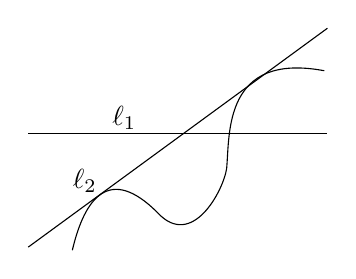
\begin{tikzpicture}[scale=1]
		\draw (1.84, 7.52).. controls (2, 8.2) and (2.32, 8.6) .. (2.92, 8).. controls (3.36, 7.52) and (3.76, 8.28) .. (3.8, 
		8.56).. controls (3.84, 9) and (3.76, 10.04) .. (5.04, 9.8);
		\draw (1.28,7.56)--(5.08,10.34);
		\draw (1.28,9)--(5.08, 9);
		\node at (2.5,9.2) {$\ell_1$};
		\node at (2,8.4) {$\ell_2$};
	\end{tikzpicture}
    \caption{}
    \end{minipage}
    \begin{minipage}[t]{0.48\textwidth}
    \centering
	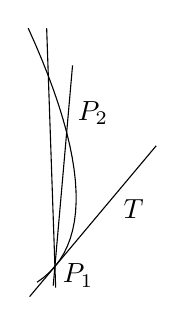
\begin{tikzpicture}[scale=1]
		\begin{scope}[rotate = 50]
			\draw plot[domain=-0.3:2.1,variable=\t] ({\t}, {\t*\t/2});
			\draw (-0.5,0)--(2,0);
			\node at (0.1,-0.3) {$P_1$};
			\node at (1.2,-0.3) {$T$};	
			\draw (-0.2,-0.14)--(1.4*1.5,1.96/2*1.5);
			\draw (-0.2,-0.18)--(1.8*1.25,3.24/2*1.25);
			\node at (1.8,1.96/2-0.1) {$P_2$};
		\end{scope}
	\end{tikzpicture}
    \caption{}
    \end{minipage}
\end{figure}

下面我们来阐述一般曲线的切线的定义,并由这个定义
推导圆锥曲线的切线方程.

\begin{blk}
   {定义} 设$P_1$为曲线上一点,过$P_1$引割线$P_1P_2$交曲线
于另一点$P_2$, 当$P_2$沿曲线无限趋近于点$P_1$时,割线$P_1P_2$
的极限位置$P_1T$叫做曲线在$P_1$点的切线(图6.17). 
\end{blk}

已知椭圆$\frac{x^2}{a^2}+\frac{y^2}{b^2}=1$,
设$P_1(x_1,y_1)$是椭圆上一定点,$P_2(x_2,y_2)$是椭圆上任
一点,则椭圆的割线$P_1P_2$的方程为
\begin{equation}
    y-y_1=\frac{y_2-y_1}{x_2-x_1}(x-x_1)=\frac{y^2_2-y^2_1}{(x_2-x_1)(y_2+y_1)}(x-x_1)
\end{equation}
由于点$P_1(x_1,y_1)$, $P_2(x_2,y_2)$都在已给的椭圆上,
所以
\[y^2_1=b^2\left(1-\frac{x^2_1}{a^2}\right),\qquad y^2_2=b^2\left(1-\frac{x^2_2}{a^2}\right)\]
两式相减得
\[y_2^2-y_1^2=\frac{b^2}{a^2}(x^2_2-x^2_1)\]
代入(6.12)化简即可得
\[y-y_1=\frac{b^2}{a^2}\cdot \frac{x_2+x_1}{y_2+y_1}(x-x_1)\]
当$P_2$与$P_1$重合时,即$x_2=x_1$, $y_2=y_1$, 上式变为
\[y-y_1=\frac{b^2}{a^2}\cdot \frac{x_1}{y_1}(x-x_1)\]
或
\[\frac{x_1x}{a^2}+\frac{y_1y}{b^2}=\frac{x_1^2}{a^2}+\frac{y_1^2}{b^2}\]
即:
\begin{equation}
    \boxed{\frac{x_1x}{a^2}+\frac{y_1y}{b^2}=1}
\end{equation}
(6.13)式就是椭圆$\frac{x^2}{a^2}+\frac{y^2}{b^2}=1$
在点$P_1(x_1,y_1)$的切线方程.

同理可证,双曲线
$\frac{x^2}{a^2}-\frac{y^2}{b^2}=1$
在点$P_1(x_1,y_1)$处的切线方程为
\begin{equation}
    \boxed{\frac{x_1x}{a^2}-\frac{y_1y}{b^2}=1}
\end{equation}

抛物线$y^2=2px$在点$P_1(x_1,y_1)$处的切线方程为
\begin{equation}
    \boxed{y_1y=p(x+x_1)}
\end{equation}

经过切点$P_1(x_1,y_1)$与切线垂直的直线叫做曲线在点
$P_1$的\textbf{法线}.

根据法线的定义可知,法线的方向向量可取切线的法向
量,因此可得椭圆、双曲线、抛物线的在$P_1(x_1,y_1)$点的
法线方程分别为
\begin{align}
    \frac{x-x_1}{b^2x_1}&=\frac{y-y_1}{a^2y_1}\\
    \frac{x-x_1}{b^2x_1}&=\frac{y-y_1}{-a^2y_1}\\
    \frac{x-x_1}{p}&=\frac{y-y_1}{-y_1}
\end{align}


\begin{example}
    求椭圆:$2x^2+3y^2=35$在其上一点$P(2,3)$
的切线方程.
\end{example}

\begin{solution}
    已知椭圆化为标准方程为
\[\frac{x^2}{\dfrac{35}{2}}+\frac{y^2}{\dfrac{35}{3}}=1\]
所以,已知椭圆在点$P(2,3)$的切线方程为
\[\frac{2x}{\dfrac{35}{2}}+\frac{3y}{\dfrac{35}{3}}=1\]
整理得:$4x+9y=35$
\end{solution}

\begin{example}
    设双曲线$\frac{x^2}{a^2}-\frac{y^2}{b^2}=1$
在其上任一点$P_0(x_0,y_0)$的切线与双曲线的两条渐近线分别相交于$A$、$B$两点(图6.18),求证$\triangle OAB$的面积等于常数$ab$.
\end{example}



\begin{solution}
已知双曲线在$P_0(x_0,y_0)$的切线方程为
\[\frac{x_0x}{a^2}-\frac{y_0y}{b^2}=1\]
将它分别与渐近线方程$y=-\frac{b}{a}x$,
$y=\frac{b}{a}x$联立求解,就可分别得到
\[A\left(\frac{a^2b}{bx_0+ay_0},\frac{-ab^2}{bx_0+ay_0}\right),\qquad B\left(\frac{a^2b}{bx_0-ay_0},\frac{ab^2}{bx_0-ay_0}\right)\]
所以
\[\begin{split}
    S_{\triangle OAB}&=\frac{1}{2}\begin{vmatrix}
        \frac{a^2b}{bx_0+ay_0}& \frac{-ab^2}{bx_0+ay_0}\\
        \frac{a^2b}{bx_0-ay_0}& \frac{ab^2}{bx_0-ay_0}
\end{vmatrix}\\
&=\frac{1}{2}\left(\frac{a^3b^3}{b^2x^2_0-a^2y_0^2}+\frac{a^3b^3}{b^2x^2_0-a^2y_0^2}\right)\\
&=\frac{a^3b^3}{b^2x^2_0-a^2y_0^2}=\frac{a^3b^3}{a^2b^2}=ab
\end{split}\]
\end{solution}

\begin{figure}[htp]\centering
    \begin{minipage}[t]{0.48\textwidth}
    \centering
\begin{tikzpicture}[>=latex, scale=1]
 \draw[->](-1,0)--(4,0)node[right]{$X$};
\draw[->](0,-3)--(0,3)node[right]{$Y$};    
\node at (0,0)[below left]{$O$};
\draw(3,3)--(0,0)--(3,-3);
\draw[domain=-2.5:2.5, samples=100, thick]plot({sqrt(1+\x*\x)},\x);
\draw[domain=-.5:3, samples=10, thick]plot(\x, {-0.89+1.34*\x});

\tkzDefPoints{1.5/1.12/P_0, .38/-.38/A, 2.62/2.62/B}
\tkzDrawPoints(P_0,A,B)
\tkzLabelPoints[right](P_0)
\tkzLabelPoints[left](B)
\tkzLabelPoints[below](A)

    \end{tikzpicture}
    \caption{}
    \end{minipage}
    \begin{minipage}[t]{0.48\textwidth}
    \centering
    \begin{tikzpicture}[>=latex, scale=1]
 \draw[->](-2,0)--(3,0)node[right]{$X$};
\draw[->](0,-3)--(0,3)node[right]{$Y$};    
\node at (0,0)[below left]{$O$};\node at (-.5,0)[below left]{$T$};
\draw(-.5,-2.5)--(-.5,2.5);
\draw[domain=-2.2:2.2, samples=100, thick]plot({0.5*\x*\x}, \x);      
\draw(-1,1.414)--(2.5,1.414)node[right]{$E$};
\tkzDefPoints{1/1.414/M, 0.5/0/F, 2/0/N, 2.5/1.414/E}
\tkzDrawSegments(M,F M,N)
\tkzDrawPoints(M,F,N)
\tkzLabelPoints[below](F,N)\tkzLabelPoints[above](M)
\draw[domain=-2:3, samples=100]plot(\x, {0.707*\x+0.707});  
\tkzMarkAngles[mark=none, size=.3](M,N,F F,M,N)
\tkzMarkAngles[mark=none, size=.4](N,M,E)
    \end{tikzpicture}
    \caption{}
    \end{minipage}
    \end{figure}

\begin{example}
    设$F$是抛物线$y^2=2px$的焦点,$M$是抛物线上任
    一点,$MT$是抛物线在点$M$的切线,$MN$是法线并与$X$轴相
    交于$N$点,直线$ME$平行$X$轴(图6.19),
    
    求证:$\angle FMN=\angle NME$.
\end{example}

\begin{solution}
设$M(x_1,y_1)$, 则由在$M$点的切线方程可得在
$M$点的法线方程为
\[y-y_1=-\frac{y_1}{p}(x-x_1)\]
令$y=0$,
得$N(x_1+p,0)$, 
所以
\[\overline{FN}=x_1+p-\frac{p}{2}= x_1+\frac{p}{2}\]
又由抛物线的定义可知,$\overline{MF}$等于$M$点到准线$x=-\frac{p}{2}$的距离,即
\[\overline{FM}=x_1+\frac{p}{2}\]
所以
$\overline{FN}=\overline{FM},\quad \angle FMN=\angle FNM$, 
但$\angle FNM=\angle NME$,
所以
\[\angle FMN=\angle NME\]
\end{solution}

例6.12所证结论告诉我们,如果一族平行光线照射到抛物
线上,经抛物线反射都通过焦点,抛物线这种光学性质有许
多用途,例如太阳能灶的聚光镜,把太阳光线(看作平行)
集中到焦点上,在焦点产生高温,探照灯把放在焦点处光
源发出的光线经镜面反射后成为平行光线等.

我们同样可以证明,椭圆和双曲线具有如下性质.
\begin{itemize}
    \item 椭圆的法线平分切点与两个焦点连线所成的角(图6.20).
    \item 双曲线的法线平分切点与两个焦点连线所成角的邻补角
(图6.21).
\end{itemize}

我们把证明留给同学.作为练习.
    
\begin{figure}[htp]\centering
    \begin{minipage}[t]{0.48\textwidth}
    \centering
\begin{tikzpicture}[>=latex, scale=1]
\draw[->](-2.5,0)--(2.75,0)node[right]{$X$};
\draw[->](0,-2)--(0,2.5)node[right]{$Y$};
\draw[thick](0,0) ellipse [x radius=2, y radius=1.25];        
\node at (0,0)[below left]{$O$};
\tkzDefPoints{1.5/0/F_2, -1.5/0/F_1, 1.25/0.976/M}
\tkzDrawPoints(F_1,F_2,M)\tkzLabelPoints[below](F_1,F_2)
\tkzLabelPoints[above](M)
\tkzDrawSegments(F_1,M F_2,M)
\draw[domain=-1:2.5, samples=10]plot(\x, {1.6-0.5*\x});
\draw[domain=.76:1.25, samples=10]plot(\x, {2*\x-1.524});

\tkzDefPoints{.76/0/S1}
\tkzMarkAngle[mark=none, size=.35](F_1,M,S1)
\tkzMarkAngle[mark=none, size=.45](S1,M,F_2)

    \end{tikzpicture}
    \caption{}
    \end{minipage}
    \begin{minipage}[t]{0.48\textwidth}
    \centering
    \begin{tikzpicture}[>=latex, scale=.8]
\draw[->](-2.5,0)--(4.5,0)node[right]{$X$};
\draw[->](0,-2.5)--(0,3)node[right]{$Y$};    
\draw[domain=-2:2, samples=100, thick]plot({sqrt(1+\x*\x)}, \x);
\draw[domain=-2:2, samples=100, thick]plot({-sqrt(1+\x*\x)}, \x);
\tkzDefPoints{-1.414/0/F_1, 1.414/0/F_2, 2/1.732/M}
\tkzDrawSegments(F_2,M)
\tkzDrawLines[add=.25 and .35](F_1,M)
\tkzLabelPoints[below](F_1, F_2)
\tkzDrawPoints(F_1, F_2, M)
\tkzLabelPoints[above left](M)
\node at (0,0)[below left]{$O$};
\draw[domain=.2:2.5, samples=10]plot(\x, {1.155*\x-0.577});
\draw(M)--+(-40.9:3);
\tkzDefPoints{4/0/S1, 2.828/2.15/S2}
\tkzMarkAngle[mark=none, size=.35](F_2,M,S1)
\tkzMarkAngle[mark=none, size=.5](S1,M,S2)
    \end{tikzpicture}
    \caption{}
    \end{minipage}
    \end{figure}
    
上述性质说明,椭圆和双曲线具有类似于抛物线的光学
性质,由椭圆一个焦点射出的光线照射到椭圆上,经过反射
后都通过另一焦点(图6.22),在双曲线一个焦点发出的
光线,照射到双曲线上,经过反射,会使光线散开,如同光
线从另一个焦点发出来的光线一样(图6.23).

    
\begin{figure}[htp]\centering
    \begin{minipage}[t]{0.48\textwidth}
    \centering
\begin{tikzpicture}[>=latex, scale=1]
\draw[thick](0,0) ellipse [x radius=2, y radius=1.25];        
\tkzDefPoints{1.5/0/F_2, -1.5/0/F_1}
\tkzLabelPoints[right](F_1, F_2)
\tkzDefPoints{-1/1.08/S1, -1/-1.08/S2, 0/1.25/S3, 0/-1.25/S4}
\tkzDrawSegments[->](F_1,S1 F_1,S2 F_1,S3 F_1,S4 S1,F_2  S2,F_2  S3,F_2  S4,F_2)
    \end{tikzpicture}
    \caption{}
    \end{minipage}
    \begin{minipage}[t]{0.48\textwidth}
    \centering
    \begin{tikzpicture}[>=latex, scale=1]
\draw[->](-2.5,0)--(2.5,0)node[right]{$X$};
\draw[->](0,-2)--(0,2.5)node[right]{$Y$};   
\draw[domain=-2:2, samples=100, thick]plot({sqrt(1+\x*\x)}, \x);
\draw[domain=-2:2, samples=100, thick]plot({-sqrt(1+\x*\x)}, \x);
\tkzDefPoints{-1.414/0/F_1, 1.414/0/F_2}
\tkzDefPoints{-1.2/.66/S1, -1.4/.98/S2, -1.6/1.25/S3, -1.2/-.66/S4, -1.4/-.98/S5, -1.6/-1.25/S6}
\tkzDrawSegments[dashed](F_2,S1 F_2,S2 F_2,S3 F_2,S4 F_2,S5 F_2,S6)
\tkzDrawSegments[thick,->](F_1,S1 F_1,S2 F_1,S3 F_1,S4 F_1,S5 F_1,S6)
\tkzLabelPoints[below](F_2)
\tkzLabelPoints[below left](F_1)
\node at (0,0)[below left]{$O$};
\foreach \x in {1,2,...,6}
{
    \tkzDefPointWith[linear, K=1.5](F_2,S\x) \tkzGetPoint{D\x}
\tkzDrawSegments[thick,->](S\x,D\x)
}
    \end{tikzpicture}
    \caption{}
    \end{minipage}
    \end{figure}

\begin{ex}
\begin{enumerate}
    \item 证明本小节的双曲线的切线方程(6.14).
    \item 证明本小节的抛物线的切线方程(6.15).
    \item 已知如下各曲线上一点的坐标,求在这点的切线和法线
    方程.
\begin{enumerate}
    \item $\frac{x^2}{225}+\frac{y^2}{25}=1,\qquad (9,4)$
    \item $2x^2+3y^2=14,\qquad (1,-2)$
    \item $4x^2-y^2=15,\qquad (2,-1)$
    \item $y^2=3x,\qquad (12,6)$
\end{enumerate}

    \item 求抛物线$y^2=4x$在点$(36,12)$的切线在$X$轴上的截
    距.
    \item 已知椭圆$\frac{x^2}{a^2}+\frac{y^2}{b^2}=1$
  在$P_1(x_1,y_1)$的切线与过两顶
    点$A_1,A_2$且垂直于$X$轴的两条直线分别相交于$C$、$D$
    两点,求证:$\overline{A_1C}\cdot \overline{A_2D}=b^2$.
    \item 求证:双曲线两条渐近线之间的切线段被切点等分.
\end{enumerate}
\end{ex}

\subsection{圆锥曲线的直径}
\begin{blk}
  {定义} 通过椭圆(双曲线)中心的直线,叫做\textbf{椭圆(双
曲线)的直径},与抛物线的轴平行的直线叫做\textbf{抛物线的直径}.

如果一条直线与圆锥曲线相交于两点,那么交点间的线
段叫做\textbf{圆锥曲线的弦}(图6.24).  
\end{blk}

\begin{figure}[htp]
    \centering
\begin{tikzpicture}[>=latex]
\begin{scope}
\draw[->](-2,0)--(2,0)node[right]{$X$};
\draw[->](0,-2)--(0,2)node[right]{$Y$};
\node at (0,0)[below left]{$O$};
\draw [pattern=north east lines](0,0) ellipse [x radius=1.5, y radius=1];
\draw(-2,1.5)--(2,-1.5);
\node at (0,-2.5){(1)};
\end{scope}

\begin{scope}[xshift=5cm]
    \draw[->](-1,0)--(3,0)node[right]{$X$};
\draw[->](0,-2)--(0,2)node[right]{$Y$};
\draw(0,1)--(3,1);
\node at (0,0)[below left]{$O$};
\draw[pattern=north east lines, domain=-1.5:1.5 ,samples=100, thick] plot({\x*\x},\x);
\node at (0,-2.5){(2)};
\end{scope}

\begin{scope}[yshift=-5cm]
    \draw[->](-2,0)--(2,0)node[right]{$X$};
\draw[->](0,-2)--(0,2)node[right]{$Y$};
\node at (0,0)[below left]{$O$};
\fill[pattern=north west lines, domain=-1.5:1.5 ,samples=100] plot({sqrt(1+\x*\x)},\x)--(0,1.5)--(0,-1.5)--(1.8,-1.5);
\fill[pattern=north west lines, domain=-1.5:1.5 ,samples=100] plot({-sqrt(1+\x*\x)},\x)--(0,1.5)--(0,-1.5)--(-1.8,-1.5);
\draw[domain=-1.5:1.5 ,samples=100, thick] plot({sqrt(1+\x*\x)},\x);
\draw[domain=-1.5:1.5 ,samples=100, thick] plot({-sqrt(1+\x*\x)},\x);
\node at (0,-2.5){(3)};
\draw(-1,2)--(1,-2);
\end{scope}

\begin{scope}[xshift=5cm, yshift=-5cm]
    \draw[->](-2,0)--(2,0)node[right]{$X$};
\draw[->](0,-2)--(0,2)node[right]{$Y$};
\node at (0,0)[below left]{$O$};
\node at (0,-2.5){(4)};
\draw[pattern=north east lines, domain=-1.5:1.5 ,samples=100, thick] plot({sqrt(1+\x*\x)},\x);
\draw[pattern=north east lines, domain=-1.5:1.5 ,samples=100, thick] plot({-sqrt(1+\x*\x)},\x);
\draw(-2,1)--(2,-1);

\end{scope}
\end{tikzpicture}
    \caption{}
\end{figure}


\begin{blk}
  {定理} 圆锥曲线的平行弦的中点在直径上.
\end{blk}

我们以椭圆为例加以证明,关于双曲线和抛物线的情况
留给同学作为练习.

已知椭圆$\frac{x^2}{a^2}+\frac{y^2}{b^2}=1$, 求证它的一族平行弦的中点在它的一条直径上(图6.24(1)).

\begin{proof}
    如果平行弦垂直于对称轴,那么,由椭圆的对称
性,定理显然成立.我们来证明一般情况.
设平行弦所在的平行线系方程为
$y=kx+c,\quad k\ne 0$.
代入已知椭圆方程整理得
\[(b^2+a^2k^2)x^2+2a^2kcx+a^2(c^2-b^2)=0\]
设这个二次方程的两个根为$x_1,x_2$, 则:
\[x_1+x_2=-\frac{2a^2kc}{b^2+a^2k^2}\]
因此平行弦中点的横坐标
\[x=\frac{x_1+x_2}{2}=-\frac{a^2kc}{b^2+a^2k^2}\]
代入直线系方程得中点的纵坐标
\[y=-\frac{b^2c}{b^2+a^2k^2}\]
于是
\[\frac{y}{x}=-\frac{b^2}{a^2k}\]
所以平行弦中点的坐标都在直线$y=-\frac{b^2}{a^2k}x$
上,这条直线通过椭圆中心,因此它是椭圆的直径.
\end{proof}

已知椭圆$\frac{x^2}{a^2}+\frac{y^2}{b^2}=1$的一族平行弦平行于直径$y=kx$,则直径$y=k'x,\quad \left(k'=-\frac{b^2}{a^2k}\right)$
叫做$y=kx$的\textbf{共轭直径}.

上述定理也就是说,与一条直径平行的弦的中点都在它
的共轭直径上.显然直径的共轭性是相互的(图6.25).

\begin{figure}[htp]\centering
    \begin{minipage}[t]{0.48\textwidth}
    \centering
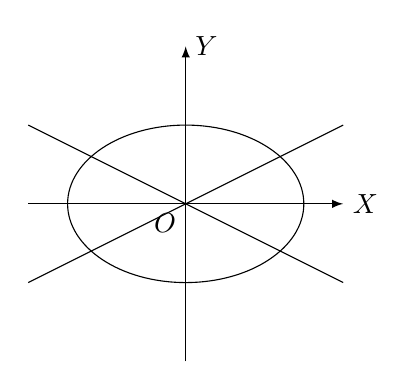
\begin{tikzpicture}[>=latex, scale=1]
\draw[->](-2,0)--(2,0)node[right]{$X$};
\draw[->](0,-2)--(0,2)node[right]{$Y$};
\node at (0,0)[below left]{$O$};
\draw (0,0) ellipse [x radius=1.5, y radius=1];
\draw(-2,1)--(2,-1);
\draw(-2,-1)--(2,1);
    \end{tikzpicture}
    \caption{}
    \end{minipage}
    \begin{minipage}[t]{0.48\textwidth}
    \centering
    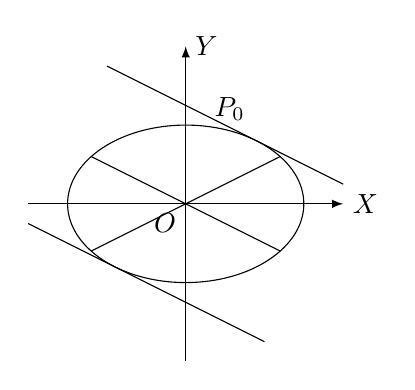
\begin{tikzpicture}[>=latex, scale=1]
\draw[->](-2,0)--(2,0)node[right]{$X$};
\draw[->](0,-2)--(0,2)node[right]{$Y$};
\node at (0,0)[below left]{$O$};
\draw (0,0) ellipse [x radius=1.5, y radius=1];
\draw[domain=-1.2:1.2, samples=10]plot(\x, {0.5*\x});
\draw[domain=-1.2:1.2, samples=10]plot(\x, {-0.5*\x});
\draw[domain=-1:2, samples=10]plot(\x, {-0.5*\x+1.25});
\draw[domain=-2:1, samples=10]plot(\x, {-0.5*\x-1.25});
\node at (.56,.93)[above]{$P_0$};
    \end{tikzpicture}
    \caption{}
    \end{minipage}
    \end{figure}

\begin{example}
    $P_0(x_0,y_0)$是椭圆$\frac{x^2}{a^2}+\frac{y^2}{b^2}=1$与它的一条
直径$y=kx$的交点,求证椭圆在$P_0(x_0,y_0)$的切线平行于
这条直径的共轭直径(图6.26).
\end{example}

\begin{proof}
    椭圆在$(x_0,y_0)$点的切线方程是$\frac{x_0x}{a^2}+\frac{y_0y}{b^2}=1$,它的斜率$k'=-\frac{x_0b^2}{a^2y_0}$,
    但$(x_0,y_0)$在已知直径上,所以
\[\frac{y_0}{x_0}=k,\qquad k'=-\frac{b^2}{a^2k}\]
又已知直径$y=kx$的共轭直径是
$y=-\frac{b^2}{a^2k}x$,所以切线
与共轭直径平行.
\end{proof}


\begin{ex}
\begin{enumerate}
    \item 对双曲线和抛物线情况证明本节定理.
    \item 已知椭圆$3x^2+4y^2=12$, 求倾角为$135^{\circ}$的椭圆平行弦
    中点所在的直线方程.
    \item 已知双曲线$2x^2-y^2=6$, 它的一族平行弦的倾角是
    $30^{\circ}$, 求这族平行弦中点所在的直线方程.
    \item 在练习2、3中写出与弦平行的直径和它的共轭直径的
    方程.
    \item 已知抛物线$y^2=6x$的一族平行弦的斜率是$1/2$, 
    求平分这族平行弦的直径方程.
    \item 设$P_0(x_0,y_0)$是双曲线
    $\frac{x^2}{a^2}-\frac{y^2}{b^2}=1$
    与它的一条直
    径$y=kx$的交点,求证:双曲线在$P_0(x_0,y_0)$的切线
    平行于这条直径的共轭直径.
\end{enumerate}
\end{ex}

\section*{习题6.1}

\addcontentsline{toc}{subsection}{习题6.1}

\begin{enumerate}
\item 在椭圆$24x^2+30y^2=720$上,求与短轴相距为5的点
的坐标.
\item 一椭圆以坐标轴为对称轴,坐标原点为对称中心且经过
点$M(\sqrt{3},-2)$, $N(-2\sqrt{3},1)$, 求此椭圆的方
程.
\item 点$P(x_1,y_1)$和点$Q(x_2,y_2)$分别位于椭圆的内部
和外部,求证
\[\frac{x_1^2}{a^2}+\frac{y_1^2}{b^2}<1,\qquad \frac{x_2^2}{a^2}+\frac{y_2^2}{b^2}>1\]
\item 已知一椭圆的准线方程是$x=\pm 8$, 短轴长等于8, 求
此椭圆的方程.
\item 已知椭圆$36x^2+100y^2=3600$, 在它上面求一点使这点
到右焦点的距离是这点到左焦点距离的4倍.
\item 已知椭圆中心在原点,它的一个焦点是$F_2(3,0)$, 求
其上一点$M(4,2.4)$到准线的距离.
\item 求下列各双曲线标准方程.
\begin{enumerate}
\item 两焦点间的距离是8, 两准线间的距离是6;
\item 已知两条准线方程是$x=\pm 3\sqrt{2}$, 两条渐近线的
夹角是直角.
\item 已知渐近线方程是$y=\pm 2x$, 两个焦点距中心的距
离是5.
\item 已知渐近线方程是$y=\pm \frac{5}{3}x$, 且双曲线通过点
$N(6,9)$.
\end{enumerate}

\item 根据下列已知条件,求双曲线$\frac{x^2}{a^2}-\frac{y^2}{b^2}=1$的渐近线
方程.
\begin{enumerate}
    \item 离心率$e=2$; 
    \item 两焦点间的距离是二准线间距离的2倍.
\end{enumerate}

\item 根据下列已知条件,求双曲线$\frac{x^2}{a^2}-\frac{y^2}{b^2}=1$的离心率.
\begin{enumerate}
    \item 两渐近线之间的夹角是$60^{\circ}$;
    \item 两渐近线之间的夹角是$90^{\circ}$.
\end{enumerate}

\item 已知等轴双曲线$x^2-y^2=8$, 求一抛物线方程使它与
已知双曲线有公共焦点且通过点$M(-5,3)$.
\item 通过点$A(2,-5)$引直线平行于双曲线$x^2-4y^2=4$的
渐近线,求此直线的方程.

\item 通过点$A(3,-1)$作双曲线$\frac{x^2}{4}-y^2=1$的弦且被$A$点
平分,求此弦的方程.
\item 求下列抛物线方程,已知
\begin{enumerate}
    \item 顶点在$(0,0)$, 焦点在$(2,0)$;
    \item 顶点在$(0,0)$, 准线是$2x+5=0$;
    \item 顶点在$(0,0)$, 准线是$2y-1=0$;
    \item 顶点在$(0,0)$, 焦点在$(0,-3/5)$.
\end{enumerate}

\item 一条抛物线顶点在原点,它的轴是$X$轴并且它通过点
$M(-1,1)$, 求它的方程.

\item 求椭圆$\frac{x^2}{6}+\frac{y^2}{3}=1$的内接正方形每边所在直线的方程.
\item 求直线$Ax+By+C=0$与椭圆$\frac{x^2}{a^2}+\frac{y^2}{b^2}=1$相切的条
件.

\item 已知椭圆$\frac{x^2}{25}-\frac{y^2}{9}=1$
的两个焦点到它的某条切线的距离之比是9, 求此切线方程.
\item 求双曲线$\frac{x^2}{8}-\frac{y^2}{9}=1$在下列各点的切线,$(2\sqrt{2},0)$, $(-4,3)$.
\item 一条双曲线在点$M(4,2)$与直线$x-y-2=0$相切.
求此双曲线的方程.
\item 求直线:$Ax+By+C=0$与双曲线
$\frac{x^2}{a^2}-\frac{y^2}{b^2}=1$相切
的条件.
\item 已知抛物线$y^2=12x$, 根据下列各条件,求它的切线方
程.
\begin{enumerate}
\item 切点的横坐标$x=3$;
\item 平行于直线$3x-y+5=0$;
\item 垂直于直线$2x+y-7=0$;
\item 与直线$4x-2y+9=0$交成$\pi/4$角.
\end{enumerate}

\item 求直线$y=kx+b$与抛物线$y^2=2px$相切的条件.
\item 直线$x+y=1$与椭圆相交于$C$和$D$两点,求弦$\overline{CD}$的
中点的坐标.
\item 已知椭圆$\frac{x^2}{a^2}+\frac{y^2}{b^2}=1$, 在其上一点$P$的切线和法线分
别与$X$轴相交于$T$点和$G$点,过焦点$F_1$、$F_2$和原点分
别作切线的垂线,设垂足分别为$V$、$U$、$K$, 过$P$点作
$X$轴的垂线,设垂足为$N$, 求证:
\begin{enumerate}
    \item $\overline{ON}\cdot \overline{OT}=a^2$
    \item $\overline{PG}\cdot \overline{OK}=b^2$
    \item $\overline{OG}=e^2\cdot \overline{ON}$
    \item $\overline{F_1V}\cdot  \overline{F_2U}=b^2$
\end{enumerate}
\end{enumerate}


\section{坐标变换}
\subsection{坐标轴的平移}
不改变坐标轴的方向和长度单位,只变换原点的位置,
这种坐标系的变换叫做\textbf{坐标轴的平移},简称\textbf{移轴}.

给定一坐标系$OXY$, 平移
坐标轴得到新坐标系$O'X'Y'$, 
下面我们来确定平面上任意一点
$P$的新坐标$(x',y')$与原坐标
$(x,y)$之间的关系(图6.27).

\begin{figure}[htp]
    \centering
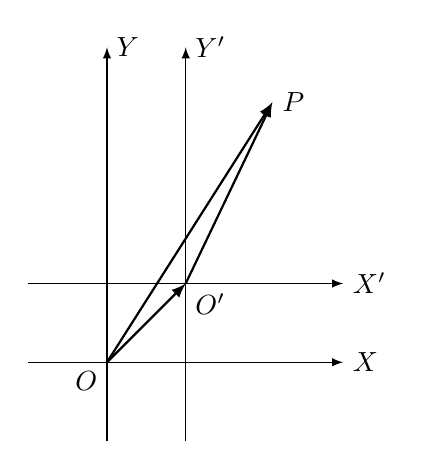
\begin{tikzpicture}[>=latex]
\draw[->](-1,0)--(3,0)node[right]{$X$};
\draw[->](-1,1)--(3,1)node[right]{$X'$};
\draw[->](0,-1)--(0,4)node[right]{$Y$};
\draw[->](1,-1)--(1,4)node[right]{$Y'$};
\node at (0,0)[below left]{$O$};
\node at (1,1)[below right]{$O'$};
\draw[->, thick](0,0)--(1,1);
\draw[->, thick](0,0)--(2.1,3.3)node[right]{$P$};
\draw[->, thick](1,1)--(2.1,3.3);
\end{tikzpicture}
    \caption{}
\end{figure}

设$O'$在坐标系$OXY$中的
坐标为$(h,k)$, 则在坐标系$OXY$中
\[\Vec{OO'}=(h,k),\qquad \Vec{OP}=(x,y),\qquad \Vec{O'P}=(x',y')\]
因为$\Vec{OP}=\Vec{OO'}+\Vec{O'P}$,所以
\[(x,y)=(h,k)+(x',y')\]
即:
\begin{equation}
    x=x'+h,\qquad y=y'+k
\end{equation}
或
\begin{equation}
    x'=x-h,\qquad y'=y-k
\end{equation}
公式(6.19), (6.20)叫做\textbf{平移公式}或\textbf{移轴公式}.


\begin{example}
    给定一坐标系$OXY$, 平移坐标轴,原点移到
    $O'(3,2)$, 求$A(5,6)$的新坐标.
\end{example}

\begin{solution}
把$A$、$O'$点的坐标代入平移公式(6.20), 得
    \[x'=5-3=2,\qquad y'=6-2=4\]
    即点$A$在新坐标系$O'X'Y'$中的坐标为$(2,4)$.     
\end{solution}



\begin{example}
    平移坐标轴,化简圆的方程$x^2+y^2+2x-6y+6=0$
\end{example}

\begin{solution}
    把已知圆的方程配方得
\begin{equation}
    (x+1)^2+(y-3)^2=4
\end{equation}
设它上面任一点的新坐标为
$(x',y')$, 平移坐标轴使
\[x'=x+1,\qquad y'=y-3\]
即:$x=x'-1,\qquad y=y'+3$,代入(6.21),得到新方程为(图6.28)
\[{x'}^2+{y'}^2=4\]
\end{solution}

\begin{figure}[htp]
    \centering
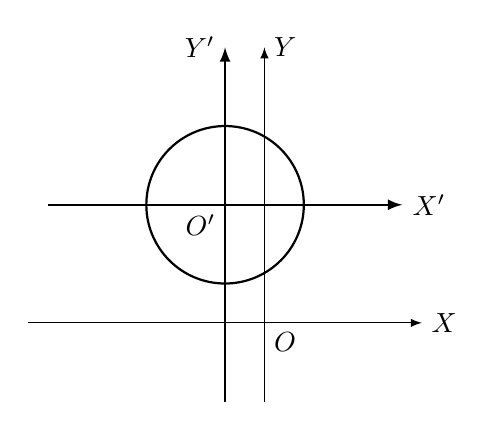
\begin{tikzpicture}[>=latex, scale=.5]
\draw[->](-6,0)--(4,0)node[right]{$X$};
\draw[->](0,-2)--(0,7)node[right]{$Y$};
\draw[->, thick](-5.5,3)--(3.5,3)node[right]{$X'$};
\draw[->, thick](-1,-2)--(-1,7)node[left]{$Y'$};
\node at (0,0) [below right]{$O$};
\node at (-1,3) [below left]{$O'$};
\draw[thick](-1,3) circle (2);
\end{tikzpicture}
    \caption{}
\end{figure}


从例6.15可以看出,适当地
变换坐标系,可以使曲线的方程简化.由于曲线的几何性质
与我们选取的坐标系无关.所以,我们研究曲线时,总是想
法选择能使曲线方程最为简单的坐标系,以便于我们研究曲
线的性质.

\begin{ex}
\begin{enumerate}
    \item 平移坐标轴,使原点移至$O'(-2,.3)$, 求下列各点的
    新坐标,并画图.
\[    A(1,2),\quad B(0,-2),\quad  C(-3,-2),\quad D(-3,-5)\]
    \item 平移坐标轴,化简下列圆的方程,并画图.
\begin{enumerate}
    \item $(x-1)^2+(y-2)^2=1$
    \item $(x+2)^2+(y-5)^2=9$
    \item $x^2+y^2+2x-6y+1=0$
\end{enumerate}

    \item 平移坐标轴,使原点移至$O'(2,-1)$, 求曲线
    $y^2+2y-4x+9=0$在新坐标系的方程.
    \item 已知直线$\ell:\; 2x+3y-5=0$, 平移坐标轴,使原点移至
    $O'\left(\frac{5}{2},0\right)$, 
求$\ell$在新坐标系中的方程.
\item 平移坐标轴,化简下列曲线方程,并画出曲线的草图.
\begin{enumerate}
    \item $\frac{(x-3)^2}{25}+\frac{(y+3)^2}{9}=1$
    \item $(x+1)^2-(y-1)^2=1$
    \item $y=4(x+3)^2-1$
\end{enumerate}
\end{enumerate}
\end{ex}

\subsection{坐标轴的旋转}
不改变坐标轴的原点和长
度单位,只是坐标轴绕原点转
一角度,这种坐标系的变换叫
做\textbf{坐标轴的旋转},简称\textbf{转轴}.

给定一坐标系,坐标轴绕
原点$O$转$\theta$角,得到一新坐标
系$OX'Y'$(图6.29). 下
面我们来确定平面上任一点$P$
的新坐标$(x',y')$与原坐标$(x,y)$之间的关系.

\begin{figure}[htp]
    \centering
    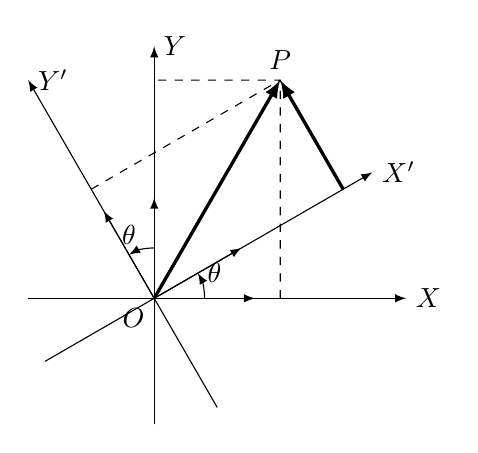
\begin{tikzpicture}[>=latex, scale=.8]
    \draw[->](-2,0)--(4,0)node[right]{$X$};
    \draw[->](0,-2)--(0,4)node[right]{$Y$};
    \draw[->](180+30:2)--(30:4)node[right]{$X'$};
\draw[->](-60:2)--(90+30:4)node[right]{$Y'$};
\draw[very thick,->](0,0)--(60:4)node[above]{$P$};        
\draw[dashed](2,0)--(60:4)--(0,2*1.732);
\draw[dashed](120:2)--(60:4);
\draw[<-, very thick](60:4)--+(-60:2);
\node at (0,0)[below left]{$O$};
\draw[->](.8,0)arc (0:30:.8)node[right]{$\theta$};
\draw[->](0,.8)arc (90:120:.8)node[above]{$\theta$};
\foreach \x in {0,30,90,120}
{
    \draw[->](0,0)--(\x:1.6);
}
    \end{tikzpicture}
    \caption{}
\end{figure}

设$\eX,\eY$和$\vec{e}_{x'},\vec{e}_{y'}$分别是两个坐标系中的基向
量,则
\[\begin{split}
    \Vec{OP}&=x\eX+y\eY=x'\vec{e}_{x'}+y'\vec{e}_{y'}\\
    \vec{e}_{x'}&=\cos\theta \eX+\sin\theta\eY\\
    \vec{e}_{y'}&=\cos\left(\frac{\pi}{2}+\theta\right)\eX+\sin\left(\frac{\pi}{2}+\theta\right)\eY=-\sin\theta\eX+\cos\theta\eY
\end{split}\]
代入上式,得
\[x\eX+y\eY=(x'\cos\theta-y'\sin\theta)\eX+(x'\sin\theta+y'\cos\theta)\eY\]
所以:
\begin{equation}
    \boxed{\begin{cases}
        x=x'\cos\theta-y'\sin\theta\\
        y=x'\sin\theta+y'\cos\theta
    \end{cases}}
\end{equation}

由(6.22)解出$x',y'$得
\begin{equation}
    \boxed{\begin{cases}
        x'=x\cos\theta+y\sin\theta\\
        y'=-x\sin\theta+y\cos\theta
    \end{cases}}
\end{equation}

(6.22)式是用新坐标来表示原坐标的公式,(6.23)式是用原
坐标来表示新坐标的公式,它们统称为\textbf{旋转公式}或转轴公
式.

\begin{example}
    把坐标轴旋转$\frac{\pi}{3}$,
求点$P(-2,3)$在新坐标系中
的坐标.
\end{example}

\begin{solution}
把已知量代入旋转公式(6.23), 得
\[\begin{split}
x'&=(-2)\cdot \cos\frac{\pi}{3}+3\cdot \sin\frac{\pi}{3}=\frac{3\sqrt{3}-2}{2},\\
y'&=-(-2)\cdot\sin\frac{\pi}{3}+3\cdot \cos\frac{\pi}{3}=\frac{2\sqrt{3}+3}{2}
\end{split}\]
所以,$P$点的新坐标是
$\left(\frac{3\sqrt{3}-2}{2}, \; \frac{2\sqrt{3}+3}{2}\right)$
\end{solution}

\begin{example}
    把坐标轴旋转$\frac{\pi}{4}$,
求曲线$xy=1$
在新坐标系中的方程.
\end{example}


\begin{solution}
    $\theta=\frac{\pi}{4}$,代入旋转公式(6.22), 得
\[\begin{split}
    x&=x'\cos\frac{\pi}{4}-y'\sin \frac{\pi}{4}=\frac{\sqrt{2}}{2}(x'-y')\\
    y&=x'\sin\frac{\pi}{4}+y'\cos\frac{\pi}{4}=\frac{\sqrt{2}}{2}(x'+y')
\end{split}\]
代入$xy=1$, 得
\[\frac{1}{2}(x'-y')(x'+y')=1\]
即:
\[\frac{{x'}^2}{\left(\sqrt{2}\right)^2}-\frac{{y'}^2}{\left(\sqrt{2}\right)^2}=1\]
这就是曲线在新坐标系中的方
程,容易看出,它是一条等轴
双曲线(图6.30).
\end{solution}

\begin{figure}[htp]
    \centering
    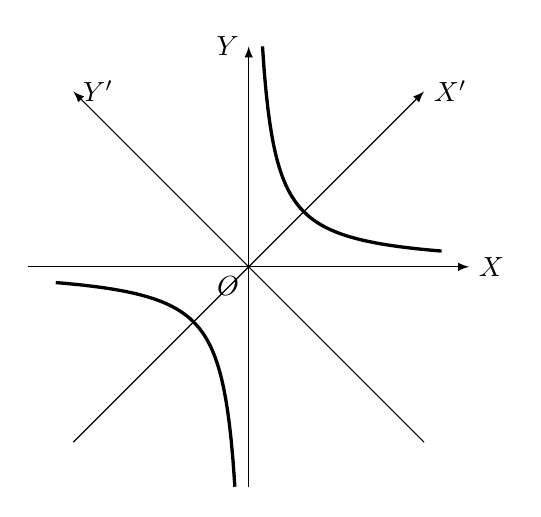
\begin{tikzpicture}[>=latex, scale=.7]
    \draw[->](-4,0)--(4,0)node[right]{$X$};
    \draw[->](0,-4)--(0,4)node[left]{$Y$};
    \draw[->](180+45:4.5)--(45:4.5)node[right]{$X'$};
\draw[->](-45:4.5)--(90+45:4.5)node[right]{$Y'$};
\draw[domain=.25:3.5, samples=100, very thick]plot(\x,{1/\x});
\draw[domain=-3.5:-.25, samples=100, very thick]plot(\x,{1/\x});     
\node at (0,0)[below left]{$O$};   
    \end{tikzpicture}
    \caption{}
\end{figure}

\begin{ex}
\begin{enumerate}
    \item 写出旋转角$\theta$为下列各值时的旋转公式(6.22)和(6.23): 
\begin{multicols}{3}
\begin{enumerate}
    \item $\theta=30^{\circ}$
    \item $\theta=-30^{\circ}$
    \item $\theta = 120^{\circ}$
    \item $\theta = 90^{\circ}$
    \item $\theta = -90^{\circ}$
    \item $\theta = 180^{\circ}$
\end{enumerate}
\end{multicols}

    \item 已知$A(2,0)$, $B(3,1)$, $C(-2,4)$. 设旋转角
    $\theta = \frac{\pi}{4}$, 
    求它们在新坐标系中的坐标.
    \item 设旋转角$\theta=45^{\circ}$, 写出下列曲线在新坐标系中的方程:
    \begin{multicols}{2}
        \begin{enumerate}
    \item $x+y=0$
\item  $x^2+y^2=4$
\item $3x^2-10xy+3y^2+8=0$
\end{enumerate}
\end{multicols}
\end{enumerate}
\end{ex}

\subsection{一般的坐标变换公式}
设$OXY$, $O'X'Y'$是两个坐标系(图6.31),$O'$在
坐标系$OXY$中的坐标是$(h,k)$, 容易看出,把坐标系
$OXY$作移轴变换,把原点
$O$移到$O'(h,k)$得到坐
标系$O'XY$然后再绕
$O'$旋转$\theta$角就可得到坐标系
$O'X'Y'$, 这就说,上述的
一般的坐标变换是平移与旋
转的合成.下面我们来确
定,平面上任意一点$P$的新
坐标$(x',y')$与原坐标$(x,y)$之间的关系.

\begin{figure}[htp]
    \centering
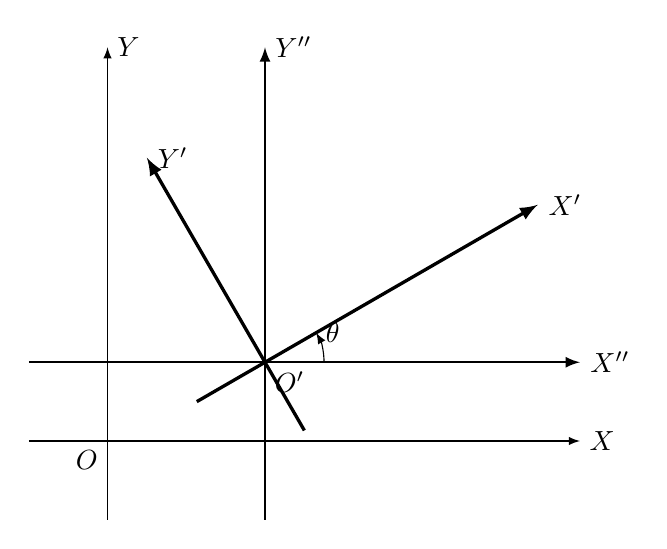
\begin{tikzpicture}[>=latex]
    \draw[->,  thick](-3,0)--(4,0)node[right]{$X''$};
    \draw[->,  thick](0,-2)--(0,4)node[right]{$Y''$};
    \draw[->, very thick](180+30:1)--(30:4)node[right]{$X'$};
\draw[->, very thick](-60:1)--(90+30:3)node[right]{$Y'$};   
\draw[->](-3,-1)--(4,-1)node[right]{$X$};
\draw[->](-2,-2)--(-2,4)node[right]{$Y$};

\node at (0,0)[below right]{$O'$};
\node at (-2,-1)[below left]{$O$};
\draw[->](.75,0)arc (0:30:.75)node[right]{$\theta$};
\end{tikzpicture}

    \caption{}
\end{figure}


设 $OXY$ 经过移轴后得到的坐标系为$O'XY$
(图6.31),则由平移公式,得
\begin{equation}
\begin{cases}
    x=x''+h\\
    y=y''+k
\end{cases}
\end{equation}
再由旋转公式,得
\begin{equation}
    \begin{cases}
        x''=x'\cos\theta-y'\sin\theta\\
        y''=x'\sin\theta+y'\cos\theta
    \end{cases}
\end{equation}
把(6.25)代入(6.24),得
\begin{equation}
    \boxed{\begin{cases}
        x=x'\cos\theta-y'\sin\theta+h\\
        y=x'\sin\theta+y'\cos\theta+k
    \end{cases} } 
\end{equation}

由(6.26)式解出$x',y'$又可得
\begin{equation}
\boxed{\begin{cases}
    x'=(x-h)\cos\theta+(y-k)\sin\theta\\
    y'=-(x-h)\sin\theta+(y-k)\cos\theta
\end{cases} }
\end{equation}
(6.26), (6.27)两个公式就是\textbf{一般的坐标变换公式}.公式(6.26)是
通过新坐标来表示原坐标,公式(6.27)是通过原坐标来表示新
坐标.

\begin{example}
    已知直线$x+y-2=0$, 
平移坐标轴,使原点移到
$O'(1,1)$, 再旋转$\left(-\frac{\pi}{4}\right)$角,
求直线$\ell$在新坐标系$O'X'Y'$中
的方程(图6.32).
\end{example}

\begin{figure}[htp]
    \centering
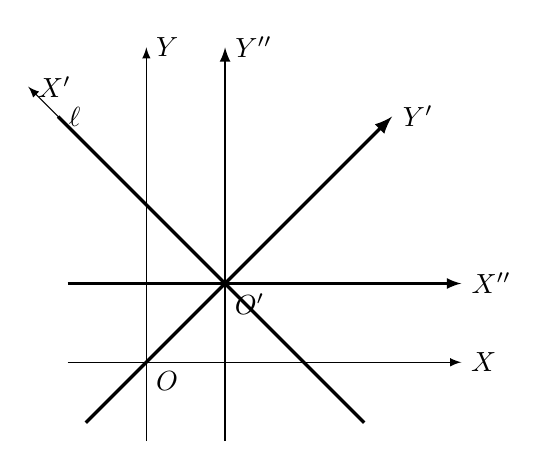
\begin{tikzpicture}[>=latex]
    \draw[->,  thick](-2,0)--(3,0)node[right]{$X''$};
    \draw[->,  thick](0,-2)--(0,3)node[right]{$Y''$};
    \draw[->, very thick](180+45:2.5)--(45:3)node[right]{$Y'$};
\draw[very thick](-45:2.5)--(90+45:3)node[right]{$\ell$};  
\draw[->](0,0)--(-2.5,2.5)node[right]{$X'$};
\draw[->](-2,-1)--(3,-1)node[right]{$X$};
\draw[->](-1,-2)--(-1,3)node[right]{$Y$};

\node at (0,0)[below right]{$O'$};
\node at (-1,-1)[below right]{$O$};
\end{tikzpicture}

    \caption{}
\end{figure}

\begin{solution}
把已知量代入变换公式(6.27), 得
\[\begin{split}
 x&=x'\cos\left(-\frac{\pi}{4}\right)-y'\sin\left(-\frac{\pi}{4}\right)+1=\frac{\sqrt{2}}{2}(x'+y')+1\\
y&=x'\sin\left(-\frac{\pi}{4}\right)+y'\cos\left(-\frac{\pi}{4}\right)+1=\frac{\sqrt{2}}{2}(-x'+y')+1   
\end{split}\]
代入方程$x+y=2$得:$$y'=0$$
这就是直线$\ell$在新坐标系中的方程.
\end{solution}

\begin{example}
    讨论线性分式函数$y=\frac{2x+1}{x-1}$
    的图象.
\end{example}

\begin{solution}
    原式可化为 $xy-2x-y-1=0$, 为了求得这个方程的图象,我们希望选择一个新坐标系,使
    图象在新坐标系中有较简单的方程.我们考虑移轴变换,
\[x=x'+h,\qquad y=y'+k\]
代入原方程,得
\[x'y'+(k-2)x'+(h-1)y'+hk-2h-k-1=0\]
如果取$h=1$, $k=2$, 上述方程变为
\[x'y'=3\]
这就是图象在新坐标系
$O'X'Y'$中的方程,由例6.17可知它是以新坐标系
的坐标轴为渐近线的等轴双
曲线(图6.33).
\end{solution}

\begin{figure}[htp]
    \centering
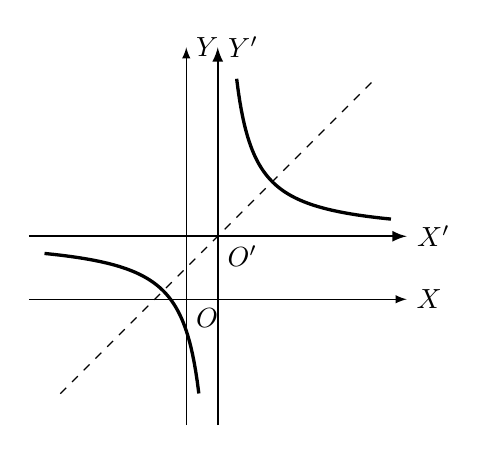
\begin{tikzpicture}[>=latex, scale=.4]
    \draw[->, thick](-6,0)--(6,0)node[right]{$X'$};
    \draw[->](-6,-2)--(6,-2)node[right]{$X$};
    \draw[->, thick](0,-6)--(0,6)node[right]{$Y'$};
    \draw[->](-1,-6)--(-1,6)node[right]{$Y$};
\draw[dashed](-5,-5)--(5,5);
\draw[domain=.6:5.5, samples=100, very thick]plot(\x,{3/\x});
\draw[domain=-5.5:-.6, samples=100, very thick]plot(\x,{3/\x});    
\node at (0,0)[below right]{$O'$};
\node at (-1,-2)[below right]{$O$};
\end{tikzpicture}
    \caption{}
\end{figure}



\begin{ex}
\begin{enumerate}
    \item 写出下列平移坐标轴,使原点移到$(h,k)$, 再旋转$\theta$角的一般坐标变换公式:
\begin{enumerate}
    \item $(h,k)=(1,1),\qquad \theta=\frac{\pi}{4}$
    \item $(h,k)=(-5,-3),\qquad \theta=120^{\circ}$
    \item $(h,k)=(0,3),\qquad \theta=-\frac{\pi}{2}$
\end{enumerate}

\item 给定坐标系$OXY$, 移轴使原点移到$O'(2,1)$, 再旋
    转$\frac{\pi}{4}$
    角,写出曲线在新坐标系中的方程:
\begin{enumerate}
    \item $2x-y-3=0$
    \item $x^2+6xy+y^2-10x-14y+9=0$
\end{enumerate}
\item     讨论线性分式函数$y=\frac{x+1}{x-1}$
的图象.
\item 取两条互相垂直的直线$x+2y+1=0$, $2x-y-3=0$, 
作新坐标轴,写出坐标变换公式.
\end{enumerate}
\end{ex}

\section*{习题6.2}
\addcontentsline{toc}{subsection}{习题6.2}


\begin{enumerate}
    \item 给定坐标系$OXY$, 已知$P(2,1)$, 移轴将原点分别移
    到下列各点,求$P$点的新坐标.
\begin{multicols}{3}
    \begin{enumerate}
        \item $(0,3)$
        \item $(3,4)$
        \item $(-2,-6)$
    \end{enumerate}
\end{multicols}

    \item 一定点$P$在坐系$OXY$与$O'X'Y'$中的坐标分别是
    $(2,5)$, $(-4,3)$且两坐标系的坐标轴方向相同,
    试求每一坐标系的原点相对于另一坐标系中的坐标.
    \item 利用配方因式分解证明下列各方程都表示一对直线,并
    作平移变换,化简这些方程:
\begin{enumerate}
\item $x^2-y^2-4x+6y-5=0$
\item $4x^2-9y^2+8x+18y-5=0$
\item $4x^2-16y^2-12x+9=0$
\end{enumerate}

    \item 转轴到怎样的角度后,才可使点$(2,0)$的两个坐标分
    量相等.
    \item 利用移变换消去方程$xy-x-y=1$中的一次项.
    \item 证明:方程$x^2+y^2=r^2$不因旋转坐标轴而变形.
    \item 取两条互相垂直的直线
  \[  ax+by+c_1=0,\qquad -bx+ay+c_2=0\]
    作新坐标系的坐标轴,建立新旧坐标系的变换公式.
    \item 取直线$x+y=0$, $x-y=0$, 分别为新坐标系的
    $X'$轴和$Y'$轴,求在新坐标系下曲线$x^2-y^2=a^2$的方程.
\end{enumerate}

\section{一般二元二次方程的讨论}
\subsection{在坐标变换下二元二次方程系数的变换}
一般二元二次方程可写为如下形式
\begin{equation}
    Ax^2+2Bxy+Cy^2+2Dx+2Ey+F=0
\end{equation}
方程的系数$A$、$B$、$C$中至少有一个不等于零,系数中析出
因子2, 是为了以后演算的方便.凡坐标满足方程(6.28)的点
的轨迹叫做\textbf{二次曲线}.

对方程(6.28), 我们进行平移和旋转变换,令
\[\begin{split}
    x&=x'\cos\theta-y'\sin\theta+h\\
y&=x'\sin\theta+y'\cos\theta+k
\end{split}\]
代入(6.28)式,展开合并同类项,就得到同一个二次曲线在
$O'X'Y'$坐标系中的方程为
\begin{equation}
    A'{x'}^2+2B'x'y'+C'{y'}^2+2D'x'+2E'y'+F'=0
\end{equation}
其中
\begin{equation}
\begin{split}
    A'&=A\cos^2\theta +2B\sin\theta \cos\theta +C\sin^2\theta \\
2B'&=-2A\sin\theta \cos\theta +2B(\cos^2\theta -\sin^2\theta)+2C\sin\theta \cos\theta\\
 &=2B\cos2\theta-(A-C)\sin2\theta \\
C'&=A\sin^2\theta -2B\cos\theta \sin\theta +C\cos^2\theta \\
D'&=2Ah\cos\theta +2B(k\cos\theta +h\sin\theta )+2Ck\sin\theta\\
&\qquad +2D\cos\theta +2E\sin\theta \\
E'&=-2Ah\sin\theta +2B(h\cos\theta -k\sin\theta)+2Ck\cos\theta\\
&\qquad  -2D\sin\theta +2E\cos\theta \\
F'&=Ah^2+2Bhk+Ck^2+2Dh+2Ek+F
\end{split}
\end{equation}

上述关系式(6.30), 骤看起来是有些繁琐的,但稍加分析
我们不难看出以下几点:
\begin{enumerate}
\item 一般二元二次方程,经坐标变换后,仍是二元二
次方程,这就是说,上述二次曲线的定义与坐标系的选取无
关.
\item 在(6.30)中,令$h=k=0$, 也就是坐标系只作旋
转变换,这时二次项系数和一次项系数一般都发生改变,而
常数项不变.新方程(6.29)中的二次项系数$A',B',C'$只与
原方程(6.28)中二次项系数和转角$\theta$有关,而与原方程中
的一次项系数和常数无关;新方程(6.29)中一次项系数只与原
方程(6.28)中一次项系数及转角有关,而与二次项系数和常数
无关.
\item 在(6.30)中,令$\theta=0$, 也就是坐标系只作平移变
换,这时二次项系数不变,即
\[A=A',\qquad B=B',\qquad C=C'\]
而一次项系数和常数项一般都要改变,且
\begin{equation}
    \begin{split}
D'&=2Ah+2Bk+2D\\
E'&=2Bh+2Ck+2E        
    \end{split}
\end{equation}
\end{enumerate}

最后让我们来证明,在一般坐标变换下,新方程(6.29)与
原方程(6.28)的系数有如下关系:
\begin{enumerate}
    \item $A+C=A'+C'$
    \item $B^2-AC={B'}^2-A'C'$
\end{enumerate}

\begin{proof}
\begin{enumerate}
    \item \[\begin{split}
 A'+C'&=A\cos^2\theta +2B\sin\theta \cos\theta 
    +C \sin^2\theta +A\sin^2\theta
    \\
    &\qquad -2B\sin\theta \cos\theta +C\cos^2\theta\\
    &=A(\cos^2\theta+\sin^2\theta)+C(\sin^2\theta+\cos^2\theta)\\
    &=A+C       
    \end{split}\]
    \item \[\begin{split}
A'-C'&=(A-C)\cos2\theta+2B\sin2\theta \\
(2B')^2+(A'-C')^2&=(2B)^2+(A-C)^2        
    \end{split}\]
    即
\[\begin{split}
    {B'}^2-A'C'&=\frac{1}{4}\left[(2B)^2+(A-C)^2-(A'+C')^2\right]\\
    &=\frac{1}{4}\left[(2B)^2+(A-C)^2-(A+C)^2\right]\\
    &=B^2-AC
\end{split}\]
\end{enumerate}
\end{proof}

由以上证明可知,\textbf{$A+C$和$B^2-AC$都是二元二次方
程在一般坐标变换下不变的量}.

\begin{ex}
\begin{enumerate}
    \item 对方程(6.28)作旋转变换,如果使方程(6.29)中$B'=0$, 
    求证:$(A'-C')^2=(A-C)^2+4B^2$.
    \item 对方程(6.28)作平移变换,如果使方程(6.29)中,消去各一
    次项,求证:
\[F=\frac{-\begin{vmatrix}
    A&B&D\\B&C&E\\D&E&F
\end{vmatrix}}{B^2-AC}\]
\end{enumerate}
\end{ex}

\subsection{一般二元二次方程的化简}
这节,我们来研究,如何选取适当的坐标系,使二次曲
线的方程有较简单的形式.

\subsubsection{用平移变换消去二元二次方程中各一次项}
由(6.31)式可知,对一般二元二次方程,若要在新
坐标系中消去各一次项,只要作平移变换选取$(h,k)$使
\[\begin{cases}
   Ah+Bk+D=0\\
Bh+Ck+E=0
\end{cases}\]
在$B^2-AC\ne 0$时,此方程组有唯一一组解$(h,k)$, 我们
将坐标原点移到$(h,k)$, 就可使二次曲线在新坐标系中的
方程中$D'=E'=0$. 在$B^2-AC=0$时,若$A:B=B:C
=D:E$, 方程组有无穷多解,若$A:B=B:C\ne D:E$, 
方程组无解,在后一种情况出现时,我们可先用下面(二)中
介绍的方法去化简方程.

\begin{example}
    平移坐标轴,化简方程
$2x^2+3y^2-8x+6y-7=0$
并画出新坐标系和方程的曲线.
\end{example}

\begin{solution}
    令$x=x'+h$, $y=y'+k$, 代入已知方程,得
\[2(x'+h)^2+3(y'+k)^2-8(x'+h)+6(y'+k)-7=0\]
就是,
\[2{x'}^2+3{y'}^2+(4h-8)x'+(6k+6)y'+2h^2+3k^2
-8h+6k-7=0\]
令$4h-8=0$, $6k+6=0$,解得
$h=2$, $k=-1$, 代入方程(6.28),得
\[2{x'}^2+3{y'}^2=18\quad \Rightarrow\quad \frac{{x'}^2}{9}+\frac{{y'}^2}{6}=1\]
这是椭圆的标准方程,对原
坐标系来说,它的中心在$O'(2,-1)$, 它的长轴和
短轴分别在直线$y=-1$, 
$x=2$上,它的长轴长是6, 短轴长是$2\sqrt{6}$. 新坐标和曲线如图6.34所示.
\end{solution}

\begin{figure}[htp]\centering
    \begin{minipage}[t]{0.48\textwidth}
    \centering
    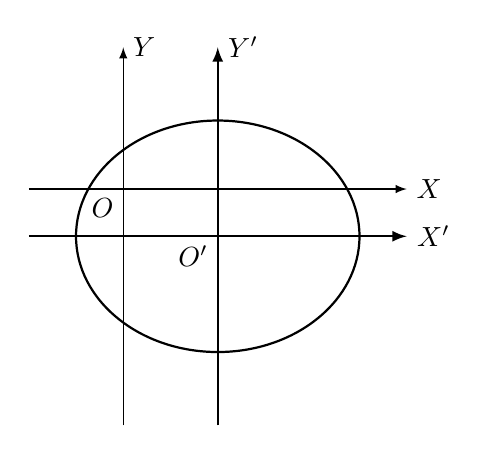
\begin{tikzpicture}[>=latex, scale=.6]
        \draw[->, thick](-4,0)--(4,0)node[right]{$X'$};
        \draw[->](-4,1)--(4,1)node[right]{$X$};
        \draw[->, thick](0,-4)--(0,4)node[right]{$Y'$};
        \draw[->](-2,-4)--(-2,4)node[right]{$Y$};
    \node at (0,0) [below left]{$O'$};\node at (-2,1) [below left]{$O$};
    \draw[thick](0,0)ellipse[x radius= 3 , y radius=2.45 ];
       
    \end{tikzpicture}
    \caption{}
    \end{minipage}
    \begin{minipage}[t]{0.48\textwidth}
    \centering
    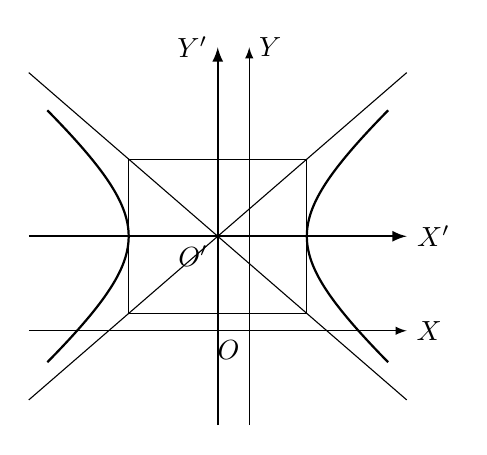
\begin{tikzpicture}[>=latex, scale=.4]
        \draw[->, thick](-6,0)--(6,0)node[right]{$X'$};
  \draw[->](-6,-3)--(6,-3)node[right]{$X$};
  \draw[->, thick](0,-6)--(0,6)node[left]{$Y'$};
  \draw[->](1,-6)--(1,6)node[right]{$Y$};

\draw[domain=-4:4, samples=100, thick]plot({sqrt(8+1.33*\x*\x)},\x);
\draw[domain=-4:4, samples=100, thick]plot({-sqrt(8+1.33*\x*\x)},\x);

\draw[domain=-6:6, samples=10]plot(\x,{0.866*\x});
\draw[domain=-6:6, samples=10]plot(\x,{-0.866*\x});
\draw(-2.828,-2.45) rectangle(2.828,2.45);
\node at (0,0) [below left]{$O'$};\node at (1,-3) [below left]{$O$};
      
    \end{tikzpicture}
    \caption{}
    \end{minipage}
    \end{figure}


\begin{example}
    平移坐标轴,化简方程
$3x^2-4y^2+6x+24y-57=0$
并画出新坐标系和方程的曲线.
\end{example}

\begin{solution}
    把已知方程按$x,y$配方,得
\[3(x+1)^2-4(y-3)^2=24\]
令$x'=x+1$, $y'=y-3$,代入上面方程,
得:
\[3{x'}^2-4{y'}^2=24 \quad \Rightarrow\quad 
\frac{{x'}^2}{8}-\frac{{y'}^2}{6}=1\]
这是双曲线的标准方程,
新坐标系和曲线如图6.35所示.
\end{solution}

\subsubsection{用旋转变换,消去(6.28)中的$xy$项}

由关系式(6.30), 对一般二元二次方程,若要在
新坐标系中使得方程不含$x'y'$项,只要选取$\theta$角,使
\[2B=2Bcos2\theta -(A-C)\sin\theta=0\]
即
\[\cot 2\theta=\frac{A-C}{2B},\qquad \left(0<\theta<\frac{\pi}{2}\right)\]
把坐标轴旋转由上式所决定的$\theta$角,就可使二次曲线在
新坐标系中的方程不含$x'y'$项.

\begin{example}
    利用坐标轴旋转化简二次方程
$8x^2+4xy+5y^2-36=0$
并画出它的图形.
\end{example}

\begin{solution}
\[\cot 2\theta=\frac{A-C}{2B}=\frac{8-5}{4}=\frac{3}{4}\]
由于$\cos2\theta$与$\cot2\theta$同号,所以
\[\begin{split}
    \cos2\theta&=\frac{\frac{3}{4}}{\sqrt{1+\left(\frac{3}{4}\right)^2}}=\frac{3}{5}\\
    \sin\theta&=\sqrt{\frac{1-\frac{3}{5}}{2}}=\frac{1}{\sqrt{5}}\\
    \cos\theta&=\sqrt{\frac{1+\frac{3}{5}}{2}}=\frac{2}{\sqrt{5}}\\
\end{split}\]
因此,可令旋转变换为
\[x=\frac{2}{\sqrt{5}}x'-\frac{1}{\sqrt{5}}y',\qquad y=\frac{1}{\sqrt{5}}x'+\frac{2}{\sqrt{5}}y'\]
代入原方程化简,得
\[9{x'}^2+4{y'}^2=36\]
这是一个椭圆,长轴在$Y'$轴上.

根据$\sin\theta=\frac{1}{\sqrt{5}}$,
得旋转角$\theta\approx 26^{\circ}34'$, 它的图形如
图6.36所示.
\end{solution}

\begin{figure}[htp]
    \centering
    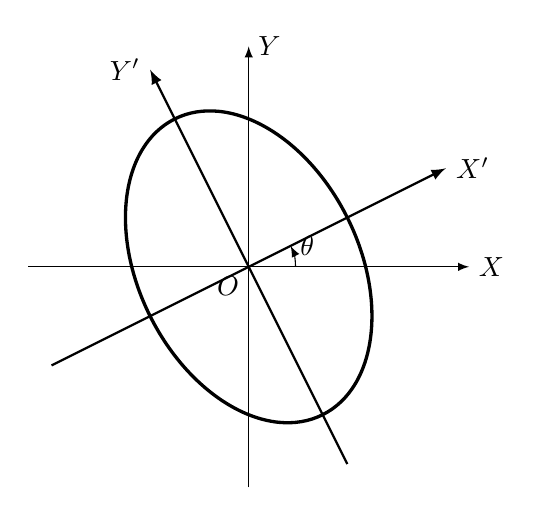
\begin{tikzpicture}[>=latex, scale=.7]
        \draw[->, thick](-180+26.56:4)--(26.56:4)node[right]{$X'$};
  \draw[->](-4,0)--(4,0)node[right]{$X$};
  \draw[->, thick](-90+26.56:4)--(26.56+90:4)node[left]{$Y'$};
  \draw[->](0,-4)--(0,4)node[right]{$Y$};

  \draw[very thick, rotate=26.56](0,0) ellipse[x radius=2, y radius=3];
  \node at (0,0) [below left]{$O$};
\draw[->](.85,0) arc (0:26.56:.85)node[right]{$\theta$};        
    \end{tikzpicture}
    \caption{}
\end{figure}

\begin{ex}
\begin{enumerate}
    \item 平移坐标轴,化简下列各二次方程
\begin{enumerate}
\item $x^2+y^2-2x+2y+3=0$
\item $9x^2+4y^2-36x+16y+16=0$
\item $2x^2-4y^2+4x+4y-1=0$
\item $xy-6x-8y+20=0$
\end{enumerate}

    \item 旋转坐标轴,化简下列各二次方程
\begin{enumerate}
     \item $x^2+12xy+9y^2-16=0$
    \item $x^2-2xy+y^2+2x-4y+3=0$
\end{enumerate}    

    \item 化简下列各二次方程
\begin{enumerate}
    \item $5x^2+6xy+5y^2-4x+4y-4=0$
    \item $9x^2+4xy+6y^2+12x+36y+44=0$
\end{enumerate}
\end{enumerate}
\end{ex}

\subsection{一般二元二次方程的讨论}
由前节可知,一些二元二次方程,经一般坐标变换
后可化为圆锥曲线的标准方程,这节我们对二元二次方程作
一般性的讨论,看看如何根据二次曲线的方程来判断它的形
状和位置.

给定二次曲线
\begin{equation}
 Ax^2+2Bxy+Cy^2+2Dx+2Ey+F=0   
\end{equation}
我们总可通过转轴,选取适当的坐标系$OX'Y'$, 使二次曲
线的方程在这个新系中不含$x'y'$项,由于转轴后方程(6.32)
中的常数项不变,新方程可写为
\begin{equation}
    A'{x'}^2+C'{y'}^2+2D'x'+2E'y'+F=0
\end{equation}
下面分两种情况讨论:
\begin{enumerate}
    \item $A'$、$C'$都不等于零(即$A'C'\ne 0$).再作平
移变换,消去一次项,由于移轴后方程(6.33)中的二次项系数
不变,所以新方程可写为
\begin{equation}
    A'{x''}^2+C'{y''}^2+F'=0
\end{equation}
我们再分两种情况:
\begin{enumerate}
\item $A'$、$C'$同号(即$A'C'>0$).当$F'\ne 0$,且
$A'$、$C'$与$F'$异号时,方程的图象是椭圆;当$F'\ne 0$且
$A'$、$C'$与$F'$同号时,显然没有点的坐标满足方程(6.34), 
因此,方程的图象不存在;当$F'= 0$, 且$A'$、$C'$同号时,
显然方程的图象只有一点.
\item $A'$、$C'$异号(即$A'C'<0$).当$F'\ne 0$时,
方程(6.32)的轨迹是双曲线;当$F'= 0$时,方程(6.34)可分解
为
\[\left(x''+\sqrt{-\frac{C'}{A'}}y''\right)\cdot \left(x''-\sqrt{-\frac{C'}{A'}}y''\right)=0\]
因此,方程的轨迹是两条相交直线.
\end{enumerate}
\item $A'$、$C'$中有一个为零(即$A'C'=0$).
设$A'=0$, 则方程(6.33)变为
\begin{equation}
    C'{y'}^2+2D'x'+2E'y'+F=0
\end{equation}
作平移变换:令$x''=x'$, $y=y'+\frac{E'}{C'}$,
方程(6.35)在新坐标
系中的方程可写为
\begin{equation}
    C'{y''}^2+2D'x''+F'=0
\end{equation}
我们再分两种情况:
\begin{enumerate}
    \item $D'\ne 0$, 这时方程的图象是抛物线.
    \item $D'=0$, 当$F'\ne 0$且$C'$与$F'$异号,方程(6.36)
    变为
    \[y''\pm \sqrt{-\frac{F'}{C'}}=0\]
    这时方程的图象两条平行直线;当$F'\ne 0$且$C'$与$F'$同
号,显然没有点的坐标满足方程,这时方程(6.32)没有轨迹,当
$F'=0$时,方程(6.36)化为$y''=0$,
这时方程(6.32)表示两条重合的直线.
\end{enumerate}
\end{enumerate}


由以上讨论可知,\textbf{一般二次曲线或者是圆锥曲线(椭圆、
双曲线、抛物线),或者是两条直线(包括重合情况),
或者是一个点,或者不存在}.

一般我们把情况1中的类型(a)叫做\textbf{椭圆型方程},
类型(b)叫做\textbf{双曲线型方程};情况2中的类型叫做
\textbf{抛物线型方程}.由于在方程(6.33)中$B'=0$, 所以
\[B^2-AC={B'}^2-A'C'=-A'C'\]
这样,上面情况1中的类型(a)的条件,$A'$、$C'$同
号相当于$B^2-AC<0$; $A'$、$C'$异号相当于$B^2-AC
>0$;情况2中的条件$A'C'$中有一个为零相当于$B^2-
AC=0$. 因此,我们可不作坐标变换,直接根据$B^2-AC$
来判别二次曲线的类型.$B^2-AC$叫做一般二元二次方
程的\textbf{判别式}.

由判别式判别二次曲线的类型,我们归纳为下表.
\begin{center}
    方程$Ax^2+2Bxy+Cy^2+2Dx+2Ey+F=0$
\begin{tabular}{cccc}
\hline
判别式&类型&一般情形&特殊情形(退化二次曲线)\\
\hline
$B^2-4C<0$ &椭圆型&椭圆&一点或没有图象\\
$B^2-4C>0$ &双曲线型&双曲线&两条相交直线\\
$B^2-AC=0$&抛物线型&抛物线&两条平行或重合直线或没有图象\\
\hline
\end{tabular}
\end{center}



\begin{example}
    试判别下列方程的类型
\begin{enumerate}
    \item $x^2-3xy+2y^2-x-5y+3=0$
    \item $9x^2-6xy+y^2-4=0$
    \item $3x^2-2xy+y^2-5x-2y+34=0$
\end{enumerate}
\end{example}

\begin{solution}
\begin{enumerate}
    \item $B^2-AC=\left(\frac{3}{2}\right)^2-1\x 2=\frac{9}{4}-1>0$
因此方程是双曲线型.
\item $B^2-AC=\left(-3\right)^2-9\x 1=0$
因此方程是抛物线型.
\item $B^2-AC=\left(-1\right)^2-3\x 1=-2<0$
因此方程是椭圆型.
\end{enumerate}    
\end{solution}

\begin{example}
    判别方程
$3x^2+12xy+12y^2+10x+10y-3=0$
的类型,并画出它的图形.
\end{example}

\begin{solution}
    $B^2-AC=\left(6\right)^2-3\x 12=0$,
    因此方程是抛物线型.
作旋转变换
\[\begin{split}
    \cot2\theta&=\frac{3-12}{12}=-\frac{3}{4},\qquad 
    \cos2\theta=\frac{-\frac{3}{4}}{\sqrt{1+\left(\frac{3}{4}\right)^2}}=-\frac{3}{5}\\
    \sin\theta&=\frac{2}{\sqrt{5}},\qquad  \cos\theta=\frac{1}{\sqrt{5}},\qquad 
    \theta \approx 63^{\circ}26'
\end{split}\]
旋转公式是
\[x=\frac{1}{\sqrt{5}}(x'-2y'),\qquad y=\frac{1}{\sqrt{5}}(2x'+y')\]
代入原方程,化简得
\[15{x'}^2+6\sqrt{5}x'-2\sqrt{5}y'-3=0\]
对$x'$配方,方程可写为
\[15\left(x'+\frac{1}{\sqrt{5}}\right)^2=2\sqrt{5}\left(y'+\frac{3}{\sqrt{5}}\right)\]
作平移变换,令$x''=x'+\frac{1}{\sqrt{5}}$, $y''=y'+\frac{3}{\sqrt{5}}$,最后方程变为
\[15{x''}^2=2\sqrt{5}y''\]
这是一条抛物线(图6.37),在$OX'Y'$坐标系中,它的顶点
是$O'\left(-\frac{1}{\sqrt{5}},-\frac{3}{\sqrt{5}}\right)$
,由旋转公式容易求得,在原坐标
系$OXY$中,它的顶点是$O'(1,-1)$. $x''$轴是直线
$2x-y-3=0$, $y''$轴是直线$x+2y+1=0$.
\end{solution}

\begin{figure}[htp]
    \centering
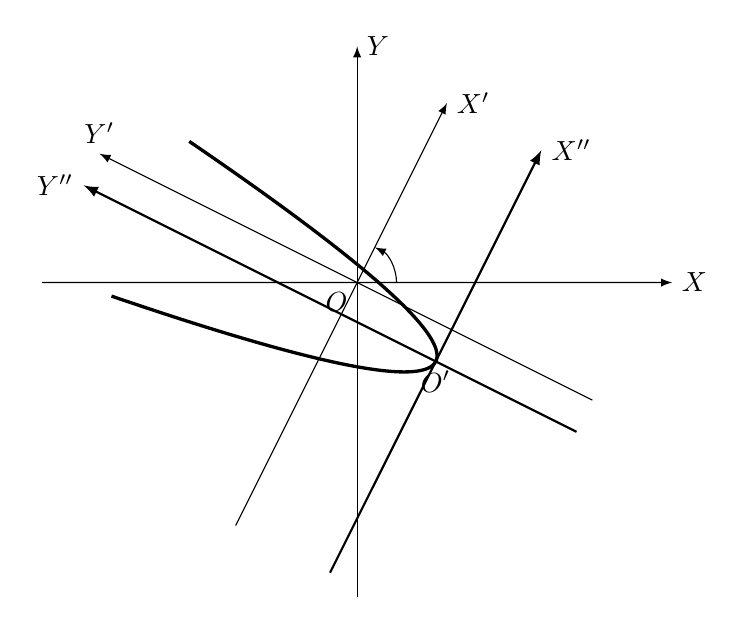
\begin{tikzpicture}[>=latex, rotate=63.43]

    \draw[->, thick](-3,0)--(3,0)node[right]{$X''$};
    \draw[->](-3,1.34)--(3,1.34)node[right]{$X'$};
    \draw[->, thick](0,-2)--(0,5)node[left]{$Y''$};
    \draw[->](0.45,-2)--(0.45,5)node[above]{$Y'$};
\draw[domain=-1.1:1.1, samples=100, very thick]plot(\x, {3.35*\x*\x});
\draw[->](0.45,1.34)--+(90-63.43:3)node[right]{$Y$};
\draw(0.45,1.34)--+(90-63.43:-4);
\draw[->](0.45,1.34)--+(-63.43:4)node[right]{$X$};
\draw(0.45,1.34)--+(-63.43:-4);
\node at (0,0)[below]{$O'$};
\node at (0.45,1.34)[below left]{$O$};
\draw[<-](0.45+.5,1.34) arc (0:-63.43:.5);
\end{tikzpicture}
    \caption{}
\end{figure}



\begin{ex}
\begin{enumerate}
    \item 试判别下列方程的类型
\begin{enumerate}
\item $16x^2-24xy+9y^2-38x-34y+71=0$
\item $x^2-5xy+13y^2-3x+21y=0$
\item $8x^2+8xy-7y^2+36y+36=0$
\item $4x^2+9y^2-16x-18y-11=0$
\item $2x^2+5xy-3y^2+3x+16y-5=0$
\end{enumerate}

    \item 判别下列方程的类型,并画出它们的图形
\begin{enumerate}
\item $5x^2-6xy+5y^2-4x-4y-4=0$
\item $7x^2-8xy+y^2+14x-8y-2=0$
\item $x^2-2xy+y^2+3x-y-4=0$
\item $3x^2-xy+5y^2-6x+y+3=0$
\item $4x^2+12xy+9y^2+2x+3y+2=0$   
\end{enumerate}

\end{enumerate}    
\end{ex}

\section*{习题6.3}
\addcontentsline{toc}{subsection}{习题6.3}

\begin{enumerate}
    \item 化简下列方程,求对称轴方程,并画出方程的图象.
\begin{enumerate}
    \item $11x^2+6xy+3y^2-12x+2y-12=0$
    \item $7x^2-8xy+y^2+14x-8y+16=0$
    \item $8x^2+8xy+2y^2-6x-3y-5=0$
    \item $x^2-2xy-6x+4y+4=0$
\end{enumerate}

\item 证明二元二次方程表示等轴双曲线或两条互相垂直的直
线的充要条件是$A+C=0$.
\item 证明抛物线$y=ax^2+bx+c\; (a\ne 0)$的对称轴平行于原
坐标轴.
\item 方程$2x^2+\lambda xy+4y^2-7x+\lambda^2y+3=0$中,$\lambda$取什么
值时,方程是:椭圆型;双曲线型;抛物
线型.
\item 设一二次曲线过点$(2,3)$, $(4,2)$, $(-1,-3)$, 且以
$(0,1)$为对称中心,求这曲线方程.
\end{enumerate}

\section*{复习题六}
\addcontentsline{toc}{section}{复习题六}

\begin{enumerate}
    \item 已知椭圆的两个焦点分别是$F_1(2,4)$、$F_2(8,4)$并经
    点$A(5,0)$, 求此椭圆方程.
    \item 两条直线$3x\pm 4y=0$都是适合下列各条件的双曲线的渐
    近线,求各双曲线方程.
\begin{enumerate}
\item 焦点在点$(0,10)$;
\item 焦点在点$(5,0)$;
\item 经过点$(7,2)$.
\end{enumerate}

    \item 求适合下列条件的抛物线的方程式.
\begin{enumerate}
    \item 顶点在点$(2,4)$, 焦点在点$(3,4)$;
    \item 经过$(0,1)$, $(2,3)$, $(5,-1)$三点且它的轴
    平行于$Y$轴;
\item     顶点在原点,准线是$x=3$.
\end{enumerate}

\item    已知椭圆$\frac{x^2}{a^2}+\frac{y^2}{b^2}=1$,直线$\overline{OP}$与$\overline{OQ}$互相垂直并与
椭圆分别相交于$P$、$Q$两点,求证:
\[\frac{1}{\overline{OP}^2}+\frac{1}{\overline{OQ}^2}=\frac{1}{a^2}+\frac{1}{b^2}\]
\item    已知$P(x_1,y_1)$和$Q(x_2,y_2)$是椭圆$b^2x^2+a^2y^2=a^2b^2$
上任意两点,又知点$L(e_{x_1},0)$, 点$M(e_{x_2},0)$; 
求证:$\overline{PM}=\overline{QL}$.
\item    已知双曲线$\frac{x^2}{a^2}-\frac{y^2}{b^2}=1$,
求证:通过点$M(h,k)$且被
$M$点平分的弦的方程是
\[\frac{hx}{a^2}-\frac{ky}{b^2}=\frac{h^2}{a^2}-\frac{k^2}{b^2}\]
\item    证明方程
\[\frac{x^2}{9+\lambda}+\frac{y^2}{5+\lambda}=1\]
当$\lambda>-5$时,表示椭圆,当$-9<\lambda<-5$时,表示双
曲线,并证明所有这些椭圆和双曲线具有公共的焦点
$(\pm 2,0)$.
\item    已知方程
\[\frac{x^2}{a^2+\lambda}+\frac{y^2}{b^2+\lambda}=1,\qquad  a>b>0\]
问$\lambda$为何值时,表示椭圆;表示双曲线.并证明
所有这些椭圆和双曲线有公共焦点.

\item 已知双曲线的轴是坐标轴,且通过点$(1,4)$和点$(-2,
7)$, 求这双曲线的方程.
\item 证明由方程$4x^2-5y^2=c$($c$为非零常数)所确定的
双曲线具有公共的渐近线.
\item 设$\alpha$是双曲线
$\frac{x^2}{a^2}-\frac{y^2}{b^2}=1$的两条渐近线的夹角,证明
$\cos\alpha=2e^{-2}-1$.
\item 已知双曲线$\frac{x^2}{a^2}-\frac{y^2}{b^2}=1$, 如果与双曲线在$P$点的切线
与两条渐近线分别相交于$E$、$F$, 求证:
\begin{enumerate}
    \item $P$点是$EF$的中点;
    \item $\overline{OE}\cdot \overline{OF}=a^2+b^2$.
\end{enumerate}

\item 双曲线$x^2-y^2=a^2$在$P$点的法线与坐标轴相交于$C$、
$D$两点,求证:$P$点是通过$O$、$C$、$D$三点圆的中心.
\item 已知双曲线
$\frac{x^2}{a^2}-\frac{y^2}{b^2}=1$在$P$点的法线分别与$X$轴,$Y$轴
相交于$C$、$D$两点,求证$\overline{CD}$中点的轨迹是
\[4(a^2x^2-b^2y^2)=(a^2+b^2)^2\]
\item 求证椭圆只有一个内接正方形和一个外切正方形.
\item 证明通过点$M(a,b)$的椭圆$b^2x^2+a^2y^2=a^2b^2$的弦的
中点的轨迹是
\[\frac{x^2}{a^2}+\frac{y^2}{b^2}=\frac{x}{a}+\frac{y}{b}\]
\item 从椭圆外一点$P(x_1,y_1)$引椭圆的两条切线,求证:
通过两个切点的直线方程为
\[\frac{xx_1}{a^2}+\frac{yy_1}{b^2}=1\]

\item 证明:在过椭圆焦点弦的两个端点处的切线相交在椭圆
的准线上.
\item 求抛物线$y^2=8ax$和$x^2=ay$在公共点切线之间的交
角.
\item 求椭圆$\frac{x^2}{6}+\frac{y^2}{3}=1$
的外切正方形的边长.
\item 已知椭圆的轴平行于坐标轴且与$X$轴相切于点$(7,0)$, 
与$Y$轴相切于点$(0,4)$. 求这椭圆的方程.
\item 在抛物线$x^2=ay\; (a>0)$上求一点$N$, 使它到$M(0,ka)$
($k>0$且为定值)的距离最小;又当$a$变化时,求$N$点的
轨迹.
\item 求抛物线$4x^2+4x+3y-2=0$的顶点和焦点的坐标及其
对称轴和准线方程.
\item 证明:任何一个以椭圆$\frac{x^2}{a^2}+\frac{y^2}{b^2}=1$
的互为共轭直径的端点为顶点的平行四边形的面积都等
于常数$2ab$. 
\item 证明:外切椭圆的矩形,其对角线之长等于定量,
\item 试证明在抛物线上三点$P_1$、$P_2$、$P_3$各引切线,这三
条切线所围成的三角形面积等于$\triangle P_1P_2P_3$面积的一
半.
\item 判定下列二次曲线的类型,并把它们化为标准方程.
\begin{enumerate}
    \item $8x^2+4xy+5y^2+8x-16y-16=0$
    \item $x^2-4xy-2y^2+10x+4y=0$
    \item $4x^2-4xy+y^2+4x-2y=0$
\end{enumerate}
\end{enumerate}


